The goal of the analysis is to search for a direct indication of \gls{LFV} in the decay of Z bosons using data from proton proton collision measured at \gls{CMS}. Beside the \gls{LFV} process, which is called signal, \gls{SM} processes exists, which leaves the same signature in the detector, but have different kinematic properties, they are referred to as backgrounds. To study the differences of signal and background, both are simulated using the Monte Carlo sampling (\gls{MC}). Including stastitical and systematic uncertanties arising from the measurement, in the end stastical methods are used to evaluate the simulation in comparison to real measured data. 

\section{Signal and background processes}

\subsection{$\tau$ lepton at \gls{CMS}}
\label{sec:section_3_1_1}

The $\tau$ lepton \cite{TAU} is the one of three leptons in the \gls{SM} and has a special role in comparison to electrons or muons. Due to the mean life time of 2.9$\cdot 10^{-13}$ the $\tau$ lepton decays after a flight distance of a few micrometer and leave secondary verteces in the tracker system. The $\tau$ lepton can decay leptonically with a branching ratio of $\text{BR}(\tau \to l\nu_{\tau}\nu_{l}) = 0.34$ or hadronically with a branching ratio of $\text{BR}(\tau \to \nu_{\tau} + \text{hadrons}) = 0.66$. Because of the high branching ratio of the hadronic decaying $\tau$ leptons (\gls{TAUH}), only this type of decay is considered in the analysis. The hadronic decays products, dependent on the speficic hadronic decay mode, leave jets as signature in \gls{CMS}.

\subsection{Signal process}
\label{sec:section_3_1_2}

To violate lepton flavour, the individual sum of each lepton flavour in initial and final state must be different: 

\begin{equation}
	\label{eq:eq_3_1}
	\sum_{n \text{ initial state particle}} f_{n} \neq  \sum_{n \text{ final state particle}} f_{n}
\end{equation}

In the case of a Z boson, produced via quark annilihation in a proton proton collider, three possible configuration fullfill the condition. The direct decay of a Z boson into a electron and a muon, referred to as $e\mu$ final state, into an electron and a $\tau$ lepton, referred to as $e\tau$ final state, and into a muon and a $\tau$ lepton, referred to as $\mu\tau$ final state, violate lepton flavour. \\

\begin{figure}[htp]
	\centering

	\begin{tikzpicture}[node distance=1.5cm]
		\coordinate[label=left:$q$] (q1);
		\coordinate[below=3cm of q1, label=left:$q$] (q2);
   
		\coordinate[below =1.5cm of q1] (k1); \coordinate[right =1.5cm of k1] (v1); 
		\coordinate[right =2cm of v1] (v2); \coordinate[right =1.5cm of v2] (k2);
		
		\coordinate[above=1.5 cm of k2,label=right:$e$] (l1);
		\coordinate[below=3cm of l1, label=right:$\mu$] (l2);

		\draw[fermion] (q1) -- (v1);
		\draw[fermion] (v1) -- (q2);
		\draw[photon] (v1) -- node[label=above:$Z$] {} (v2);
		\draw[fermion] (l1) -- (v2);
		\draw[fermion] (v2) -- (l2);
	\end{tikzpicture}

	\begin{tikzpicture}[node distance=1.5cm]
		\coordinate[label=left:$q$] (q1);
		\coordinate[below=3cm of q1, label=left:$q$] (q2);
   
		\coordinate[below =1.5cm of q1] (k1); \coordinate[right =1.5cm of k1] (v1); 
		\coordinate[right =2cm of v1] (v2); \coordinate[right =1.5cm of v2] (k2);
		
		\coordinate[above=1.5 cm of k2,label=right:$e$] (l1);
		\coordinate[below=3cm of l1, label=right:$\tau$] (l2);

		\draw[fermion] (q1) -- (v1);
		\draw[fermion] (v1) -- (q2);
		\draw[photon] (v1) -- node[label=above:$Z$] {} (v2);
		\draw[fermion] (l1) -- (v2);
		\draw[fermion] (v2) -- (l2);
	\end{tikzpicture}

	\begin{tikzpicture}[node distance=1.5cm]
		\coordinate[label=left:$q$] (q1);
		\coordinate[below=3cm of q1, label=left:$q$] (q2);
   
		\coordinate[below =1.5cm of q1] (k1); \coordinate[right =1.5cm of k1] (v1); 
		\coordinate[right =2cm of v1] (v2); \coordinate[right =1.5cm of v2] (k2);
		
		\coordinate[above=1.5 cm of k2,label=right:$\mu$] (l1);
		\coordinate[below=3cm of l1, label=right:$\tau$] (l2);

		\draw[fermion] (q1) -- (v1);
		\draw[fermion] (v1) -- (q2);
		\draw[photon] (v1) -- node[label=above:$Z$] {} (v2);
		\draw[fermion] (l1) -- (v2);
		\draw[fermion] (v2) -- (l2);
	\end{tikzpicture}
	
	\caption[Feynman diagram of LFV Z boson decay]{Feynman diagram of LFV Z boson decay into the $e\mu$, $e\tau$ and $\mu\tau$ final state}
	\label{fig:fig_3_1}

\end{figure}

In the detector such processes would leave an electron/muon pair, both directly originating from collisions point, for the $e\mu$ final state, and a lepton/jet pair, where the lepton originates from the collision point and the jet originate from a secondary vertex of a \gls{TAUH}.  

\subsection{Background processes}

Background processes have the same particles in the final state as the \gls{LFV}, but they originate from leptonic/semi-leptonic decays of the mother particles or from misidentification of the particles. This leads to differences in kinematic distributions, different secondary verteces or/and additional particles in the final state beside the two leptons. \\

The main irreducible background is the Drell-Yan (\gls{DY}) $Z\to\tau\tau$ process, where in the $e\mu$ final state both $\tau$ leptons decays leptonically into an electron, a muon and four neutrinos, and in the $e\tau$ and $\mu\tau$ final state one $\tau$ lepton decays leptonically into a lepton and the other one decays hadronically with three neutrinos. The leptons from the $\tau$ lepton decays originate from secondary verteces, have different angular correlation lepton coming directly from the Z boson like in the \gls{LFV} process and will in average more \gls{MET} and less momenta due to the neutrinos, which carries away the momenta undetected. Figure \ref{fig:fig_3_2} shows the Feynman diagram of the leptonic decay chain. Beside the $Z\to\tau\tau$ process, the second \gls{DY} process is $Z\to\ell\ell$, where one of the leptons $\ell$ has a misidentified lepton flavour. In this case the kinematic proporties are quite similiar to the \gls{LFV} process, because the lepton also originate from the $Z$ boson, and have no secondary verteces or neutrinos. \\


\begin{figure}[htp]
	\centering

	\begin{tikzpicture}[node distance=1.5cm]
		\coordinate[label=left:$q$] (q1);
		\coordinate[below=3cm of q1, label=left:$q$] (q2);

		\coordinate[right =1.5cm of k1] (v1); 
		\coordinate[right =2cm of v1] (v2); \coordinate[right =1.5cm of v2] (k2);
	
		\coordinate[above=1.5 cm of k2] (tau1);
		\coordinate[below=1.5cm of k2] (tau2);
	
		\coordinate[right=1.5 cm of tau1] (k3);
		\coordinate[above=1 cm of k3, ] (W1);
		\coordinate[below=1 cm of k3,label=right:$\nu_{\tau}$] (nu1);
		\coordinate[right=1.5 cm of W1] (k4);
		\coordinate[above=1 cm of k4, label=right:$\ell$] (l1);
		\coordinate[below=1 cm of k4, label=right:$\nu_{\ell}$] (nu2);
	
		\coordinate[right=1.5 cm of tau2] (k5);
		\coordinate[above=1 cm of k5,label=right:$\nu_{\tau}$] (nu3);
		\coordinate[below=1 cm of k5] (W2);
		\coordinate[right=1.5 cm of W2] (k6);
		\coordinate[above=1 cm of k6, label=right:$\ell'$] (l2);
		\coordinate[below=1 cm of k6,label=right:$\nu_{\ell'}$] (nu4);
	
		\draw[fermion] (q1) -- (v1);
		\draw[fermion] (v1) -- (q2);
		\draw[photon] (v1) -- node[label=above:$Z$] {} (v2);
		\draw[fermion] (tau1) -- node[label=above:$\tau$] {} (v2);
		\draw[fermion] (v2) -- node[label=below:$\tau$] {} (tau2);
	
   		\draw[fermion] (nu1) -- (tau1);
   		\draw[photon] (tau1) -- node[label=above:$W$] {} (W1);
   		\draw[fermion] (l1) -- (W1);
   		\draw[fermion] (W1) -- (nu2);
	
   		\draw[photon] (W2) -- node[label=below:$W$] {} (tau2);
   		\draw[fermion] (tau2) -- (nu3);
   		\draw[fermion] (l2) -- (W2);
   		\draw[fermion] (W2) -- (nu4);
	\end{tikzpicture}
	
	\caption[Feynman diagram of $Z\to\tau\tau$ decay]{Feynman diagram of $Z\to\tau\tau$ fully leptonic decay in the $e\mu$ final state}
	\label{fig:fig_3_2}
\end{figure}

One of the other backgrounds due to leptonic decay is the top/anti top production (\gls{TTBAR}), in which the top pair decays leptoncally into leptons, b-quarks and neutrinos. Like in the $Z\to\tau\tau$ process the lepton originate from secondary verteces and have different kinematic properties in comparison to the signal. Figure \ref{fig:fig_3_3} shows the Feynman diagram of the leptonic decay chain. \\


\begin{figure}[htp]
	\centering

	\begin{tikzpicture}[node distance=1.5cm]
		\coordinate[label=left:$g$] (g1);
		\coordinate[below=3cm of g1, label=left:$g$] (g2);

		\coordinate[right =1.5cm of k1] (v1); 
		\coordinate[right =2cm of v1] (v2); \coordinate[right =1.5cm of v2] (k2);
	
		\coordinate[above=1.5 cm of k2] (top1);
		\coordinate[below=1.5cm of k2] (top2);
	
		\coordinate[right=1.5 cm of tau1] (k3);
		\coordinate[above=1 cm of k3, ] (W1);
		\coordinate[below=1 cm of k3,label=right:$b$] (b1);
		\coordinate[right=1.5 cm of W1] (k4);
		\coordinate[above=1 cm of k4, label=right:$\ell$] (l1);
		\coordinate[below=1 cm of k4, label=right:$\nu_{\ell}$] (nu1);
	
		\coordinate[right=1.5 cm of tau2] (k5);
		\coordinate[above=1 cm of k5,label=right:$b$] (b2);
		\coordinate[below=1 cm of k5] (W2);
		\coordinate[right=1.5 cm of W2] (k6);
		\coordinate[above=1 cm of k6, label=right:$\ell'$] (l2);
		\coordinate[below=1 cm of k6,label=right:$\nu_{\ell'}$] (nu2);
	
		\draw[gluon] (g1) -- (v1);
		\draw[gluon] (v1) -- (g2);
		\draw[gluon] (v1) -- node[label=above:$g$] {} (v2);
		\draw[fermion] (top1) -- node[label=above:$t$] {} (v2);
		\draw[fermion] (v2) -- node[label=below:$t$] {} (top2);
	
   		\draw[fermion] (b1) -- (top1);
   		\draw[photon] (top1) -- node[label=above:$W$] {} (W1);
   		\draw[fermion] (l1) -- (W1);
   		\draw[fermion] (W1) -- (nu1);
	
   		\draw[photon] (W2) -- node[label=below:$W$] {} (top2);
   		\draw[fermion] (top2) -- (b2);
   		\draw[fermion] (l2) -- (W2);
   		\draw[fermion] (W2) -- (nu2);
	\end{tikzpicture}

	\caption[Feynman diagram of \gls{TTBAR} decay]{Feynman diagram of \gls{TTBAR} decay chain}
	\label{fig:fig_3_3}
\end{figure}

Beside the decay of fermions like the $\tau$ leptons and the tops, vector boson decays contributes the final states, which are under investigation. The possible vector bosons pairs are $ZZ$/$WW$/$WZ$. For the $WW$ pair, both $W$ bosons decays leptonically with two neutrinos, for the $ZZ$ pair both Z bosons decays leptonically, where two leptons of the four leptons are misidentified, and for the $WZ$ pair both decay leptonically, there one of the three leptons is misidentified. Figure \ref{fig:fig_3_4} shows the Feynman diagram of vector boson production. \\


\begin{figure}[htp]
	\centering
	\begin{tikzpicture}[node distance=1.5cm]
		\coordinate[label=left:$q$] (q1);
		\coordinate[right=2cm of q1] (v1);
		\coordinate[below=2.5cm of v1] (v2);
		\coordinate[left=2cm of v2, label=left:$q$] (q2);
		\coordinate[right=2cm of v1] (Z1);
		\coordinate[right=2cm of v2] (Z2);
		
		\coordinate[right=1 cm of Z1] (k1);
		\coordinate[above=1 cm of k1, label=right:$\ell/\ell$] (l1);
		\coordinate[below=1 cm of k1, label=right:$\ell/\nu_{\ell}$] (l2);
		
		\coordinate[right=1 cm of Z2] (k2);
		\coordinate[above=1 cm of k2, label=right:$\ell'/\ell'$] (l3);
		\coordinate[below=1 cm of k2, label=right:$\ell'/\nu_{\ell'}$] (l4);
		
		\draw[fermion] (q1) -- (v1);
		\draw[fermion] (v1)  -- node[label=left:$q$] {} (v2);
		\draw[fermion] (v2) -- (q2);
		\draw[photon] (v1)  -- node[label=above:$Z/W$] {} (Z1);
		\draw[photon] (v2)  -- node[label=below:$Z/W$] {} (Z2);
		
		\draw[fermion] (l1) -- (Z1);
		\draw[fermion] (Z1) -- (l2);
		\draw[fermion] (l3) -- (Z2);
		\draw[fermion] (Z2) -- (l4);
	\end{tikzpicture}

	\caption[Feynman diagram of vector boson production]{Feynman diagram of vector boson production}
	\label{fig:fig_3_4}
\end{figure}

On the other side processes exist, in which the end state particles are misidentified, like $Z\to\ell\ell$ discussed before. There are two main processes contributing. One of the processes if the single $W$ boson production in association of a quark, like shown in figure \ref{fig:fig_3_5}. The $W$ boson decays leptonically, but the quark, which leaves a jet in the detector, is misidentified as a lepton, in most cases the jet is reconstructed as a \gls{TAUH}. The other process are so-called \gls{QCD} multijet processes, which are the result of the hard interaction of the partons from the protons and leads to quarks/gluons in the final state, which jets are then misidentified as leptons. Figure  \ref{fig:fig_3_6} shows two possible Feynman diagrams contributing to the \gls{QCD} background.

\begin{figure}[htp]
	\centering
	\begin{tikzpicture}[node distance=1.5cm]
		\coordinate[label=left:$g$] (g);
		\coordinate[below=3cm of g, label=left:$q$] (q1);
		
		\coordinate[right=2cm of g] (k);
		\coordinate[below=1cm of k] (v1);
		\coordinate[below=1cm of v1] (v2);
		
		\coordinate[right=4cm of g, label=right:$q'$] (q3);
		\coordinate[right=4cm of q1] (W);

		\coordinate[right=1cm of W] (k2);
		\coordinate[above=1cm of k2, label=right:$\ell$] (l);
		\coordinate[below=1cm of k2, label=right:$\nu_{\ell}$] (nu);
		
		\draw[gluon] (g) -- (v1);
		\draw[fermion] (q1) -- (v2);
		\draw[fermion] (v2) -- node[label=right:$q'$] {} (v1);
		\draw[fermion] (v1) -- (q3);
		\draw[photon] (v2) -- node[label=below:$W$] {} (W);

		\draw[fermion] (nu) -- (W);
		\draw[fermion] (W) -- (l); 
	\end{tikzpicture}

	\caption[Feynman diagram of $W + \text{jets}$]{Feynman diagram of $W + \text{jets}$ production}
	\label{fig:fig_3_5}
\end{figure}

\begin{figure}[htp]
	\begin{minipage}{0.4\textwidth}
		\begin{tikzpicture}[node distance=1.5cm]
			\coordinate[label=left:$g$] (g1);
			\coordinate[below=3cm of g1, label=left:$g$] (g2);   			
			\coordinate[below =1.5cm of g1] (k1); \coordinate[right =1.5cm of k1] (v1); 
			\coordinate[right =2cm of v1] (v2); \coordinate[right =1.5cm of v2] (k2);
		
			\coordinate[above=1.5 cm of k2,label=right:$q$] (q1);
			\coordinate[below=3cm of q1, label=right:$q$] (q2);
	
			\draw[gluon] (g1) -- (v1);
			\draw[gluon] (v1) -- (g2);
			\draw[gluon] (v1) -- node[label=above:$g$] {} (v2);
			\draw[fermion] (q1) -- (v2);
			\draw[fermion] (v2) -- (q2);
		\end{tikzpicture}
	\end{minipage}

	\begin{minipage}{0.4\textwidth}
		\begin{tikzpicture}[node distance=1.5cm]
			\coordinate[label=left:$q$] (q1);
			\coordinate[right=2cm of q1] (v1);
			\coordinate[below=2.5cm of v1] (v2);
			\coordinate[left=2cm of v2, label=left:$q$] (q2);
			\coordinate[right=2cm of v1] (g1);
			\coordinate[right=2cm of v2] (g2);

			
			\draw[fermion] (q1) -- (v1);
			\draw[fermion] (v1)  -- node[label=left:$q$] {} (v2);
			\draw[fermion] (v2) -- (q2);
			\draw[gluon] (v1)  -- node[label=above:$g$] {} (g1);
			\draw[gluon] (v2)  -- node[label=below:$g$] {} (g2);
		\end{tikzpicture}
	\end{minipage}
	
	\caption[Feynman diagram of \gls{QCD} background]{Feynman diagram of two possible contributions to the \gls{QCD} multijet background}
	\label{fig:fig_3_6}
\end{figure}


\section{Event selection}
\label{sec:section_3_2}

From all events, which are recorded and stored by \gls{CMS}, only a fraction of them are particulary interesting regarding the search for \gls{LFV}. First the search for \gls{LFV} requires events having leptons with different flavour, and second it must be ensured the best quality of the idenfication of the particles. Because of this, a analysis specific event selection is performed, to select the events of interest. This selection is divided into two steps. The first step is the reconstruction/idenfication of the objects, where the raw detector information is evaluated the specific software tools to conclude about the type of particle. The second step is to select the reconstructed objects of interest in specific events and to set criteria in regard if quality of reconstruction. 


\subsection{Event reconstruction}
\label{sec:section_3_2_1}

Like discussed in section \ref{sec:section_2_2_4} and illustrated in figure \ref{fig:fig_2_5}, different particles leaves specific signatures in the detector systems of \gls{CMS}. This fact is used in the particle flow algorithm (\gls{PF}) \cite{PF}. The algorithm identifies objects for example electrons and photon from \gls{ECAL} entries or muons from hits in the muon chambers. With linking the information of the different detector system, for example a track in the tracker system and a matching \gls{ECAL} entries from an electron, all particles can be identified one after another.  From the combination of all reconstructed particle higher level objects like jets or \gls{MET} are reconstructed. \\

To ensure the best possible rate of right identification of the reconstructed particles, the \gls{CMS} collaboration provide multivariate analysis (\gls{MVA}) classifier for the different particles. The classifier are trained to do a binary classification of whether the particles is your wished particle or not, where information of detector systems are feeded into the training, see reference \cite{ERECO} for electrons \gls{MVA} classifier. \\

The $\tau$ leptons require more sophisicated methods to reconstruct, because of the short live time and the secondary particles originating from the decay. The \gls{TAUH} are reconstructed with the hadron-plus-strips algorithm \cite{TAURECO}. This algorithm uses information of the tracks and ECAL deposition of the hadrons originating from the decay of the $\tau$ lepton to a charged pion (1-prong), to a charged pion and a neutral pion (1-prong + $\pi^0$) and to three charged pions (3-prong). \\

Like for other objects the \gls{CMS} collobaration provides \gls{MVA} classifier for \gls{TAUH} \cite{TAURECO}. But due to reconstruction of the \gls{TAUH} from decay products, it is more prone that other objects (in general electrons/muons/jets) are misidentified as \gls{TAUH}. For this reason three different \gls{MVA} are provided to differentiate \gls{TAUH} and electrons/muons/jets. \\

Besides $\tau$ leptons, also jets need a sophistaced treatment to be identified from a particles cascasde in the calorimeter systems. Jets are reconstructed using the anti-$k_T$ algorithm \cite{ANTIKT}, which cluster all PF canditates originating from the primary vertex within a cone of \gls{dR} = 0.4. In this analysis jets are required to fulfill \gls{pT}$ > 30$ GeV and \gls{eta}$ < 4.7$ to be identified as a jet. In the analysis, due to the \gls{TTBAR} and its decay into b-quarks, the combined secondary vertex algorithm \cite{CSV} is used, which uses information about track-based lifetime information and the secondary vertex to provide a classifier to identify jets from b-quarks. 


\subsection{Selection criteria}
\label{sec:sec_3_2_2}

For the search of \gls{LFV} Z decays, events of interest have a pair of reconstructed electron/muon, electron/tau lepton or muon/tau lepton. On this reconstructed leptons qualatitive requirements are set, to maximize the confidence in the quality of the reconstruction. \\

The first requirement is the trigger decision of the \gls{HLT}, which is discussed in section \ref{sec:section_2_2_3}. There is not only one trigger decision, but many trigger decision made on the object of interest, in this analysis leptons, and on the \gls{pT} and \gls{eta}, which are online reconstucted during the trigger decision. 

\begin{description}
	\item [$e\mu$:] In this final state two so-called cross triger are used, which selects with event with a pair of electron and muons. The first trigger selects an electron with \gls{pT} $> 23$ GeV and $|$\gls{eta}$|$ $< 2.5$ and a muon with \gls{pT} $> 8$ GeV and $|$\gls{eta}$|$ $< 2.4$ and the second trigger selects an electron with \gls{pT} $> 12$ GeV and $|$\gls{eta}$|$ $< 2.5$ and a muon with \gls{pT} $> 23$ GeV and $|$\gls{eta}$|$ $< 2.4$. Two triggers are used to cover a larger phase space in \gls{pT} of both leptons, and of course only of the trigger has to make a positive decision.
	\item [$e\tau$:] In this final state on single trigger is used to select events with electrons. The trigger selects an electron with \gls{pT} $> 25$ GeV and $|$\gls{eta}$|$ $< 2.1$
	\item [$\mu\tau$:] In this final state one single trigger for selecting events with a muon and one cross trigger for selecting a pair of muon and \gls{TAUH}. The single trigger requires a muon with \gls{pT} $> 19$ GeV and $|$\gls{eta}$|$ $< 2.1$ and a \gls{TAUH} with \gls{pT} $> 20$ GeV and $|$\gls{eta}$|$ $< 2.5$ and the single trigger selects muons with \gls{pT} $> 22$ GeV and $|$\gls{eta}$|$ $< 2.1$.
\end{description}

The second requirement is set on the so-called isolation of the leptons. The isolation quantifies the energy deposition around a reconstructed object in cone defined by a specific value of \gls{dR}, where the energy deposition originating from other particles passing the detector. The definition of isolation is given by

\begin{equation}
	\label{eq:eq_3_1}
	I^{\ell} = \frac{\sum_{\text{charged}} p_{T} + \text{max}(0, \sum_{\text{neutral}} p_{T} - \frac{1}{2}\sum_{\text{charged, PU}} p_{T})}{p_T^{\ell}}  
\end{equation} 

with $\sum_{\text{charged}} p_{T}$ as sum of the scalar transverse momenta of all charged particles originating from the primary vertex, $\sum_{\text{neutral}} p_{T}$ as sum of the scalar transverse momenta of all neutral particles and $\sum_{\text{charged, PU}} p_{T}$ as sum of the scalar transverse momenta of all charged particles from secondary vertices in a cone of \gls{dR} = 0.4. In this analysis tight isolated lepton are required, which means for each final state: 

\begin{description}
	\item [$e\mu$:] For the electron an isolation of $I^{e} = 0.15$ and for the muon $I^{\mu} = 0.2$ are required. 
	\item [$e\tau$:]  For the electron an isolation of $I^{e} = 0.10$ is required. For the \gls{TAUH} a \gls{MVA} ID is used for quantifying isolation, which is trained to distinguish between quark/gluon jets. 
	\item [$\mu\tau$:]  For the muon an isolation of $I^{\mu} = 0.10$ is required. Like in the $e\tau$ final state the \gls{TAUH} has to pass the \gls{MVA} ID for isolation.
\end{description}


The third requirement is based on the identification of the particle. To ensure that the object of interest is correctly identified, a offline criteria based on measured quantities of the detectors entries are either used to set cut on this or to train a \gls{MVA} classifier, like mentioned in section \ref{sec:section_3_2_1}. The \gls{CMS} colloaboration provides recommendations for each particle, where different so-called working points for the selections are defined. This range from very loose to very tight, where a tighter working indicates a more trustworthy selection criteria. 

\begin{description}
	\item [$e\mu$:] The electron has to pass the tight \gls{MVA} idenfication criteria, the muon has to pass the medium cut based idenfication criteria. 
	\item [$e\tau$:]  The electron has to pass the tight \gls{MVA} idenfication criteria, the \gls{TAUH} has to pass the tight \gls{MVA} idenfication criteria to be distinguished from electrons and the loose \gls{MVA} idenfication criteria to be distinguished from muons.
	\item [$\mu\tau$:]  The muons has to pass the medium cut based idenfication criteria, the \gls{TAUH} has to pass the loose \gls{MVA} idenfication criteria to be distinguished from electrons and the tight \gls{MVA} idenfication criteria to be distinguished from muons.
\end{description}


\subsection{Categorization}
\label{sec:section_3_2_3}

The signal and background processes differ in their kinematics properties, which leads to region in phase space, where the signal events are concentrated, and region, which are background is dominating. This fact can be used in the statistical interpretation of the analysis, see section \ref{kappa}. A so-called categorization of the phase space is applied, which defines different region of interest in the phase space. \\

In terms of this analysis the number of jets are of interest. Like discussed in section \ref{sec:section_3_1_2}, the \gls{LFV} signal leads always to leptons with different flavour. In some cases, in the \gls{SM} this are called higher order corrections \cite{Peskin}, the quarks of the initial state can radiate quarks, which in the detector are measured to be jets. The other source of jets in the final state are quarks/gluons coming from the other constituens of the proton which broke during the proton-proton collision. The same argumentation is also true for the \gls{DY} background. This leads to a distribution of measured number of jets, which peaks at zero and decaying with higher number of jets in the final state. In comparison to that, some background have natural jets in their final state. Backgrounds like \gls{TTBAR}, W + jets and \gls{QCD} multijet have by default jets in the final state because of the properties of the interaction or the decay of the final state particles. The described jet distrubtion are shown figure \ref{fig:fig_3_7}. 

\begin{figure}[htp]
	\centering
	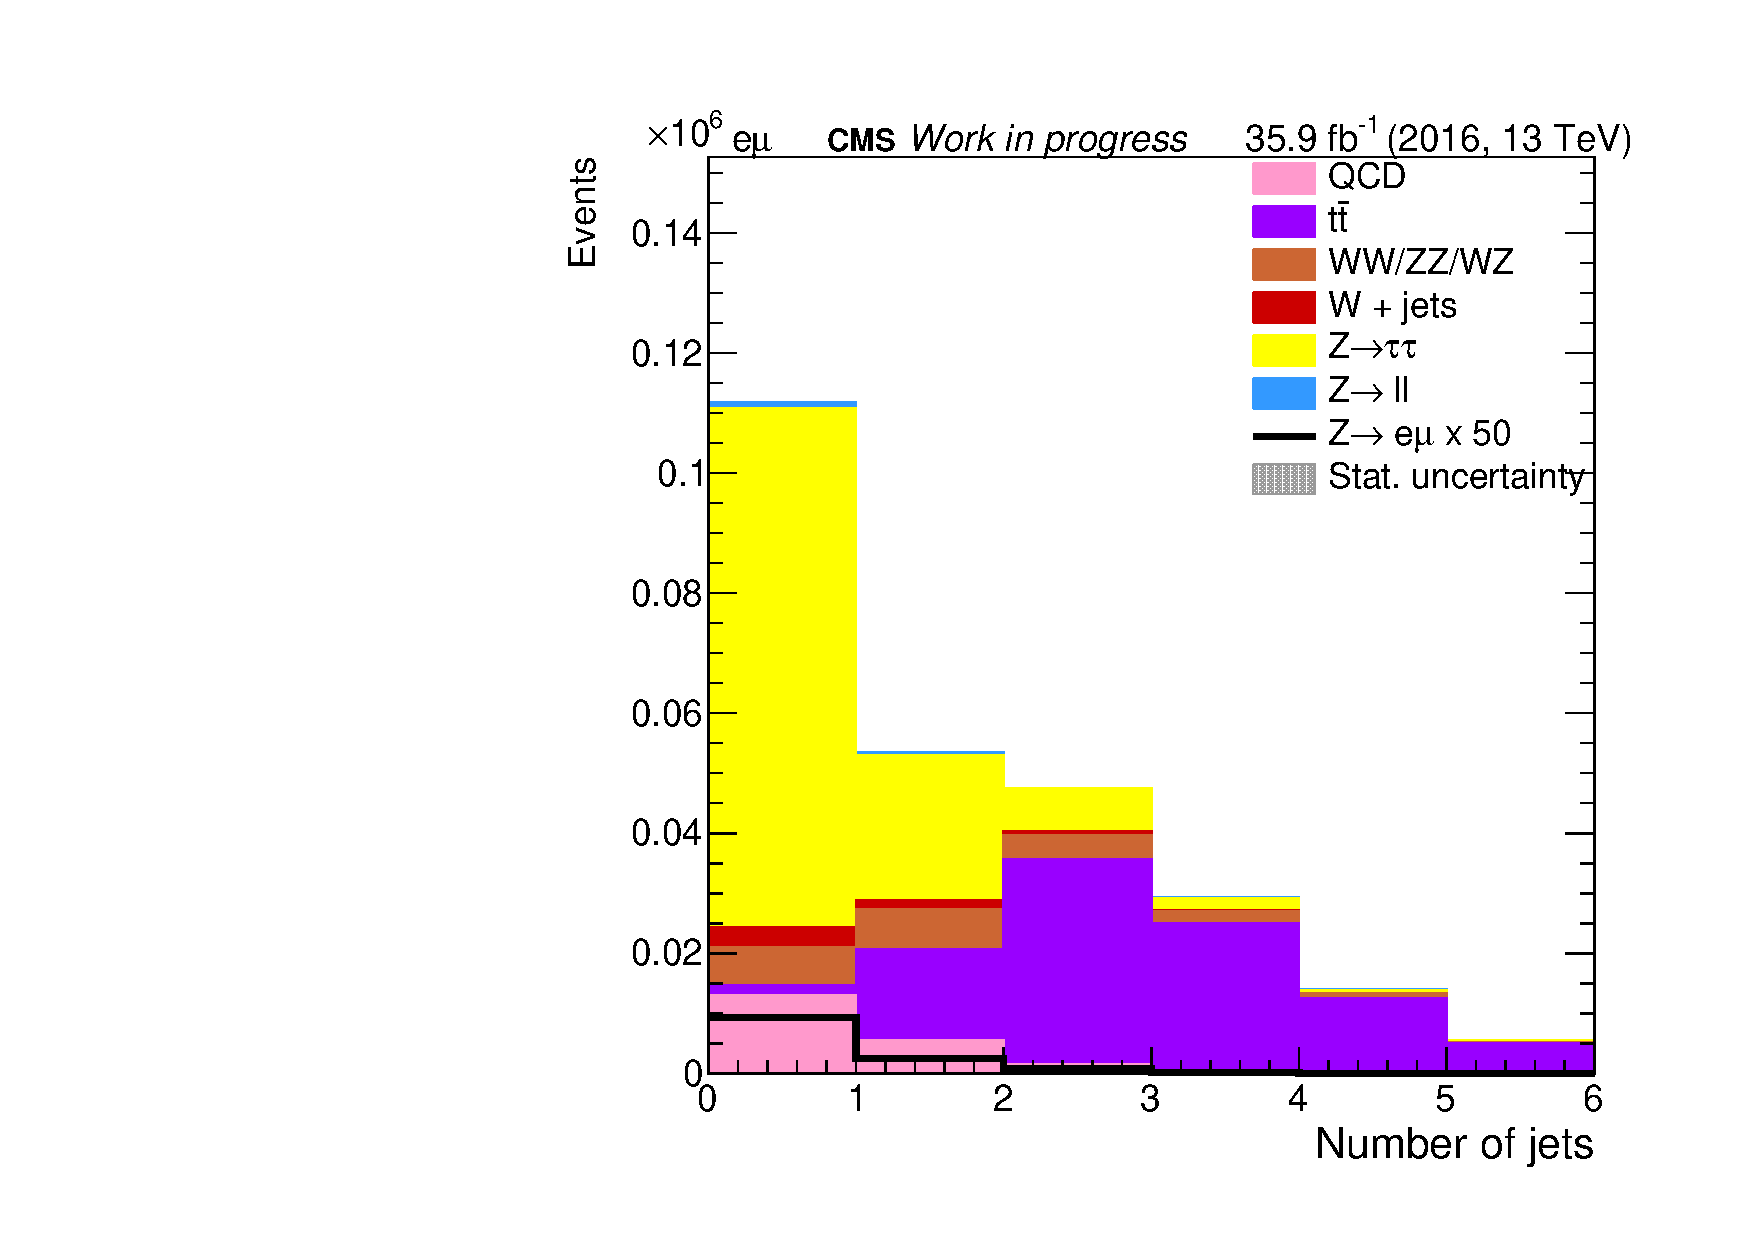
\includegraphics[width=0.4\textwidth]{plots/em/NumberOfJets.pdf}
	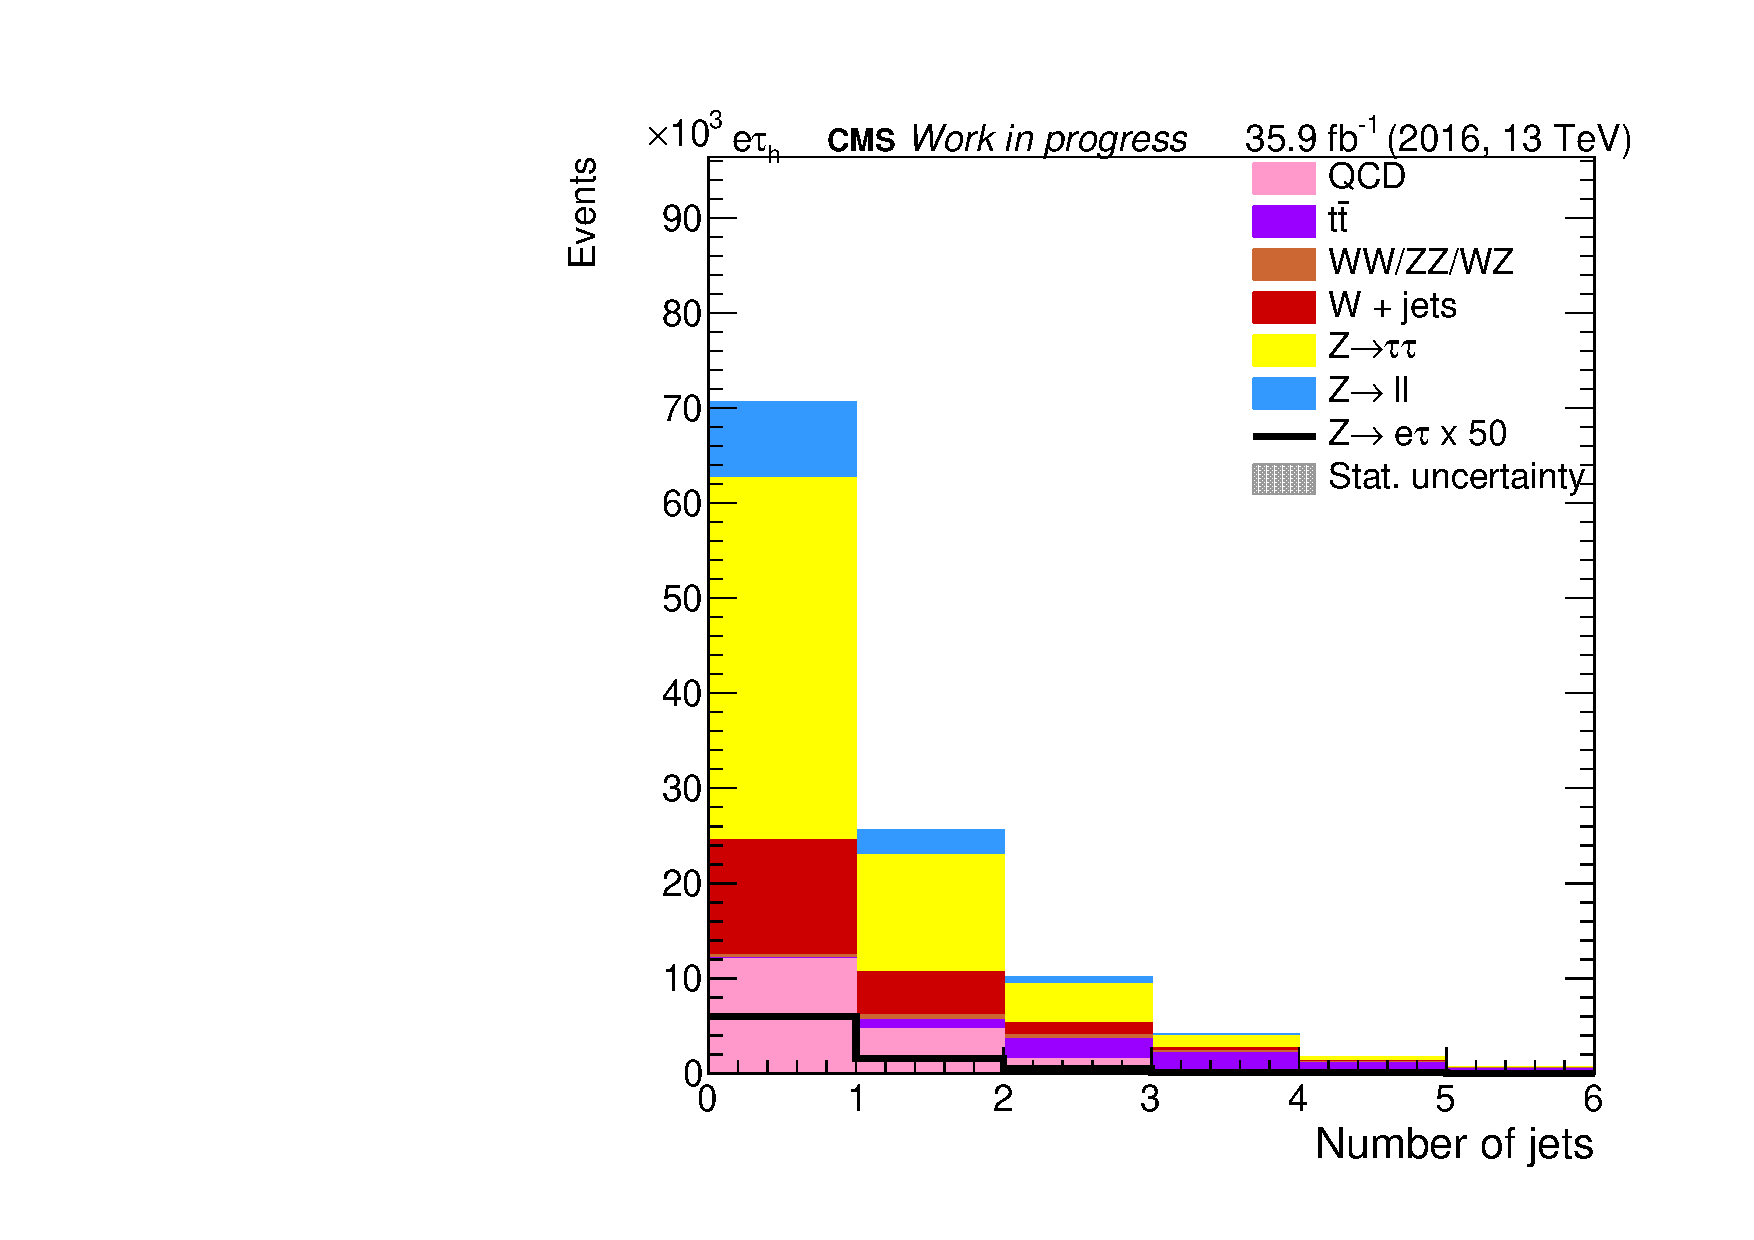
\includegraphics[width=0.4\textwidth]{plots/et/NumberOfJets.pdf}
	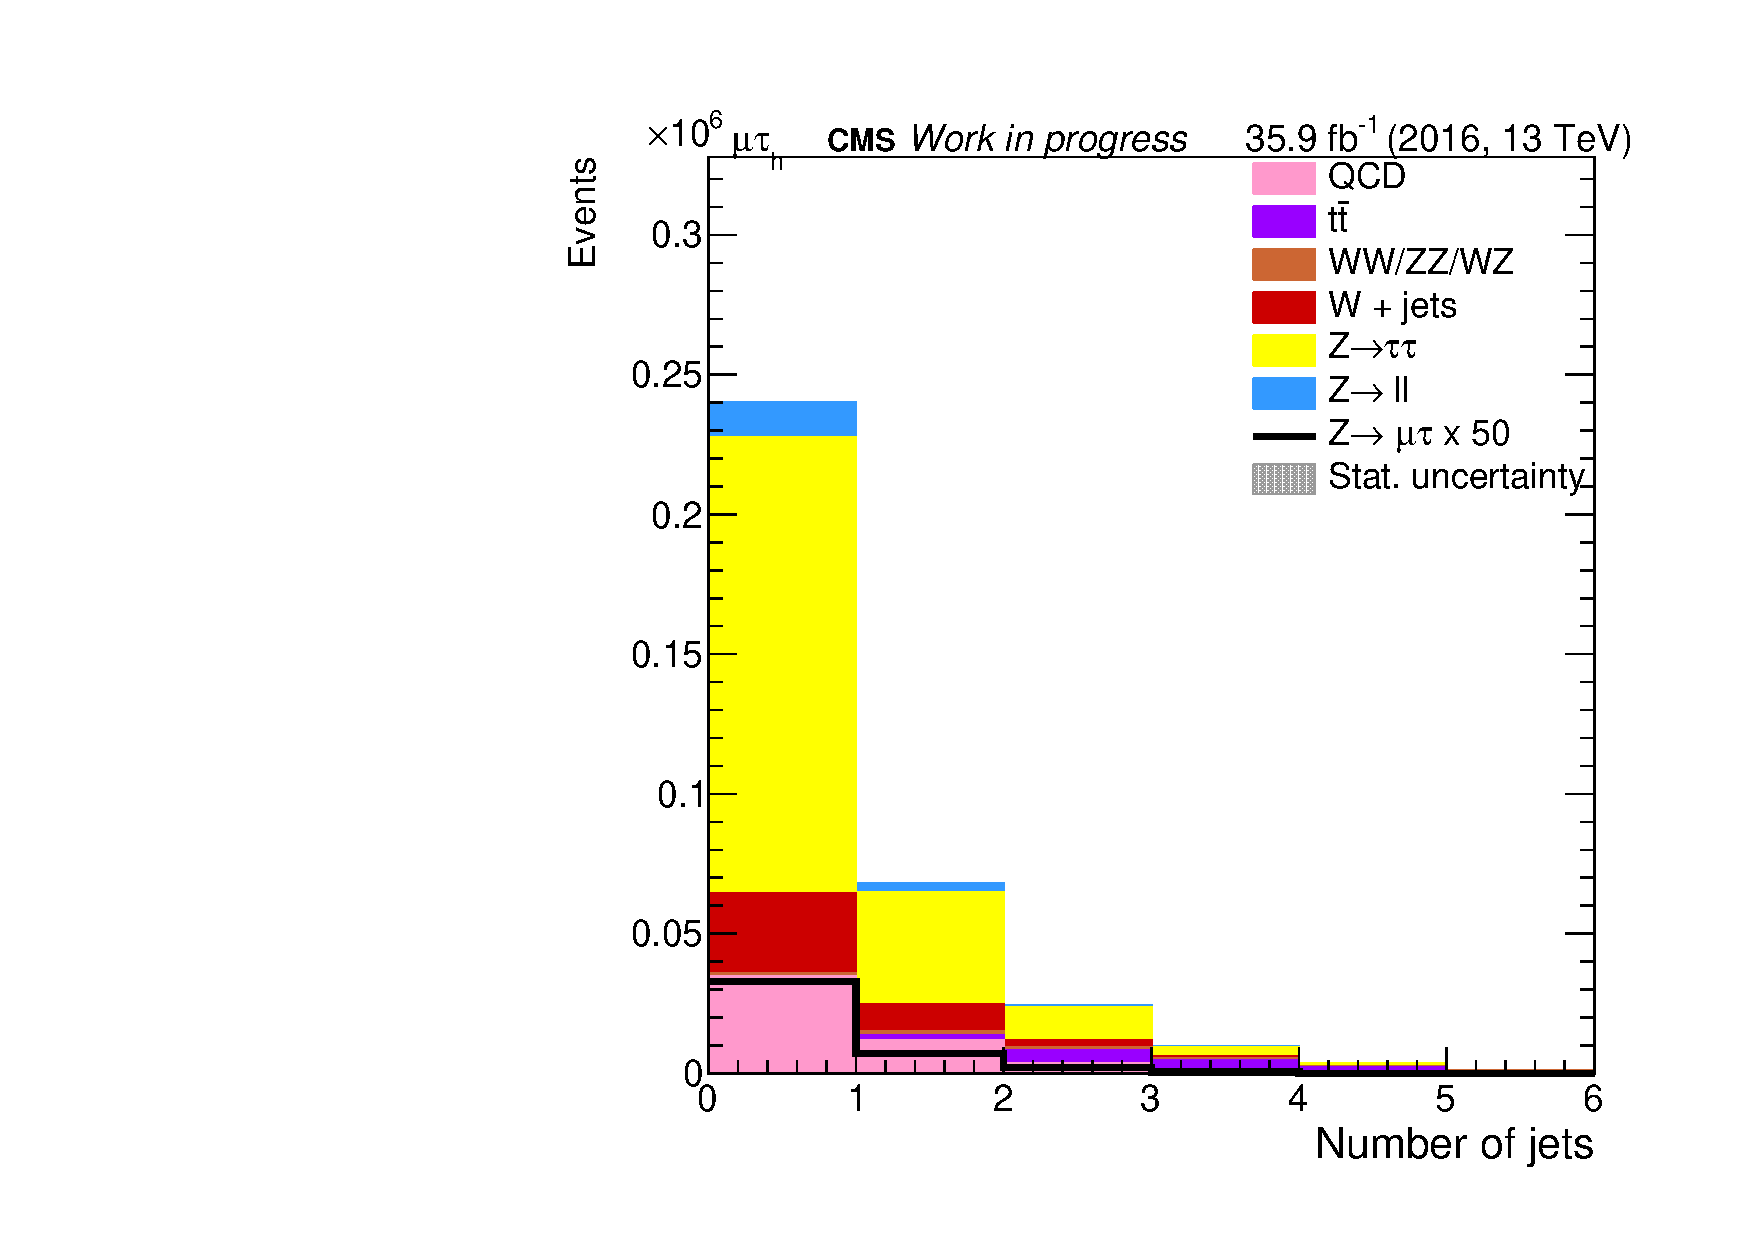
\includegraphics[width=0.4\textwidth]{plots/mt/NumberOfJets.pdf}

	\caption[Number of jet distribution of each final state]{Number of jet distribution for the final state $e\mu$, $e\tau$ and $\mu\tau$}
	\label{fig:fig_3_7}
\end{figure}

For the categorization a splitting in number of jets multiplizity is applied. Three distingued region in phase space are considered:

\begin{description}
	\item [Zero Jet category:] Event with number of jets equals to zero 
	\item [One Jet category:] Event with number of jets equals to one
	\item [Multi Jet category:] Event with number of jets more than one
\end{description}


\section{Background estimation}

The study of both signal and background processes requires the study of simulation, which can be compared with real data. The simulations of the processes are provided by the \gls{CMS} collaboration and is basically done in three steps. The first is the simulation of the physical process by using a \gls{MC} event generator, for example like madgraph \cite{MADGRAPH}, which generate mother and daugther particles with their four momenta. The second step is the simulation of proton-proton collisions, including the information of the generated particles. In the last step the detector response of \gls{CMS} is simulated by Geant4 \cite{GEANT4} using the proton-proton and the process simulation. \\

In this simulation the physical expectation for the number of events, given by formula \ref{eq:eq_2_2}, is not included yet. This expectation is calculated in the so-called background estimation, where depending on the process, the theoretical expectation and \gls{MC} simulation is used or data driven methods, using real data in signal free regions to determine backgrounds. 

\subsection{Background estimated from Monte carlo simulation}

To determine background from Z boson decays, MC simulation is used and normalized to the cross section and integrated luminosity. It is splitted into two contributions due to different decay modes of the Z. The first contribution is the $Z\to\tau\tau$ background, where $\tau_h$ are matched to generated hadronic taus and electrons/muons are matched generated leptonics taus. The second contribution is the $Z\to\ell\ell$ background, which combines events where $\tau_h$ is matched to a generated electron/muon, and all the rest. Figure \ref{fig:fig_3_8} shows the a plot of the \gls{pT} distribution of both leptons around the $Z\to\tau\tau$ mass peak. \\

\begin{figure}[htp]
	\centering
	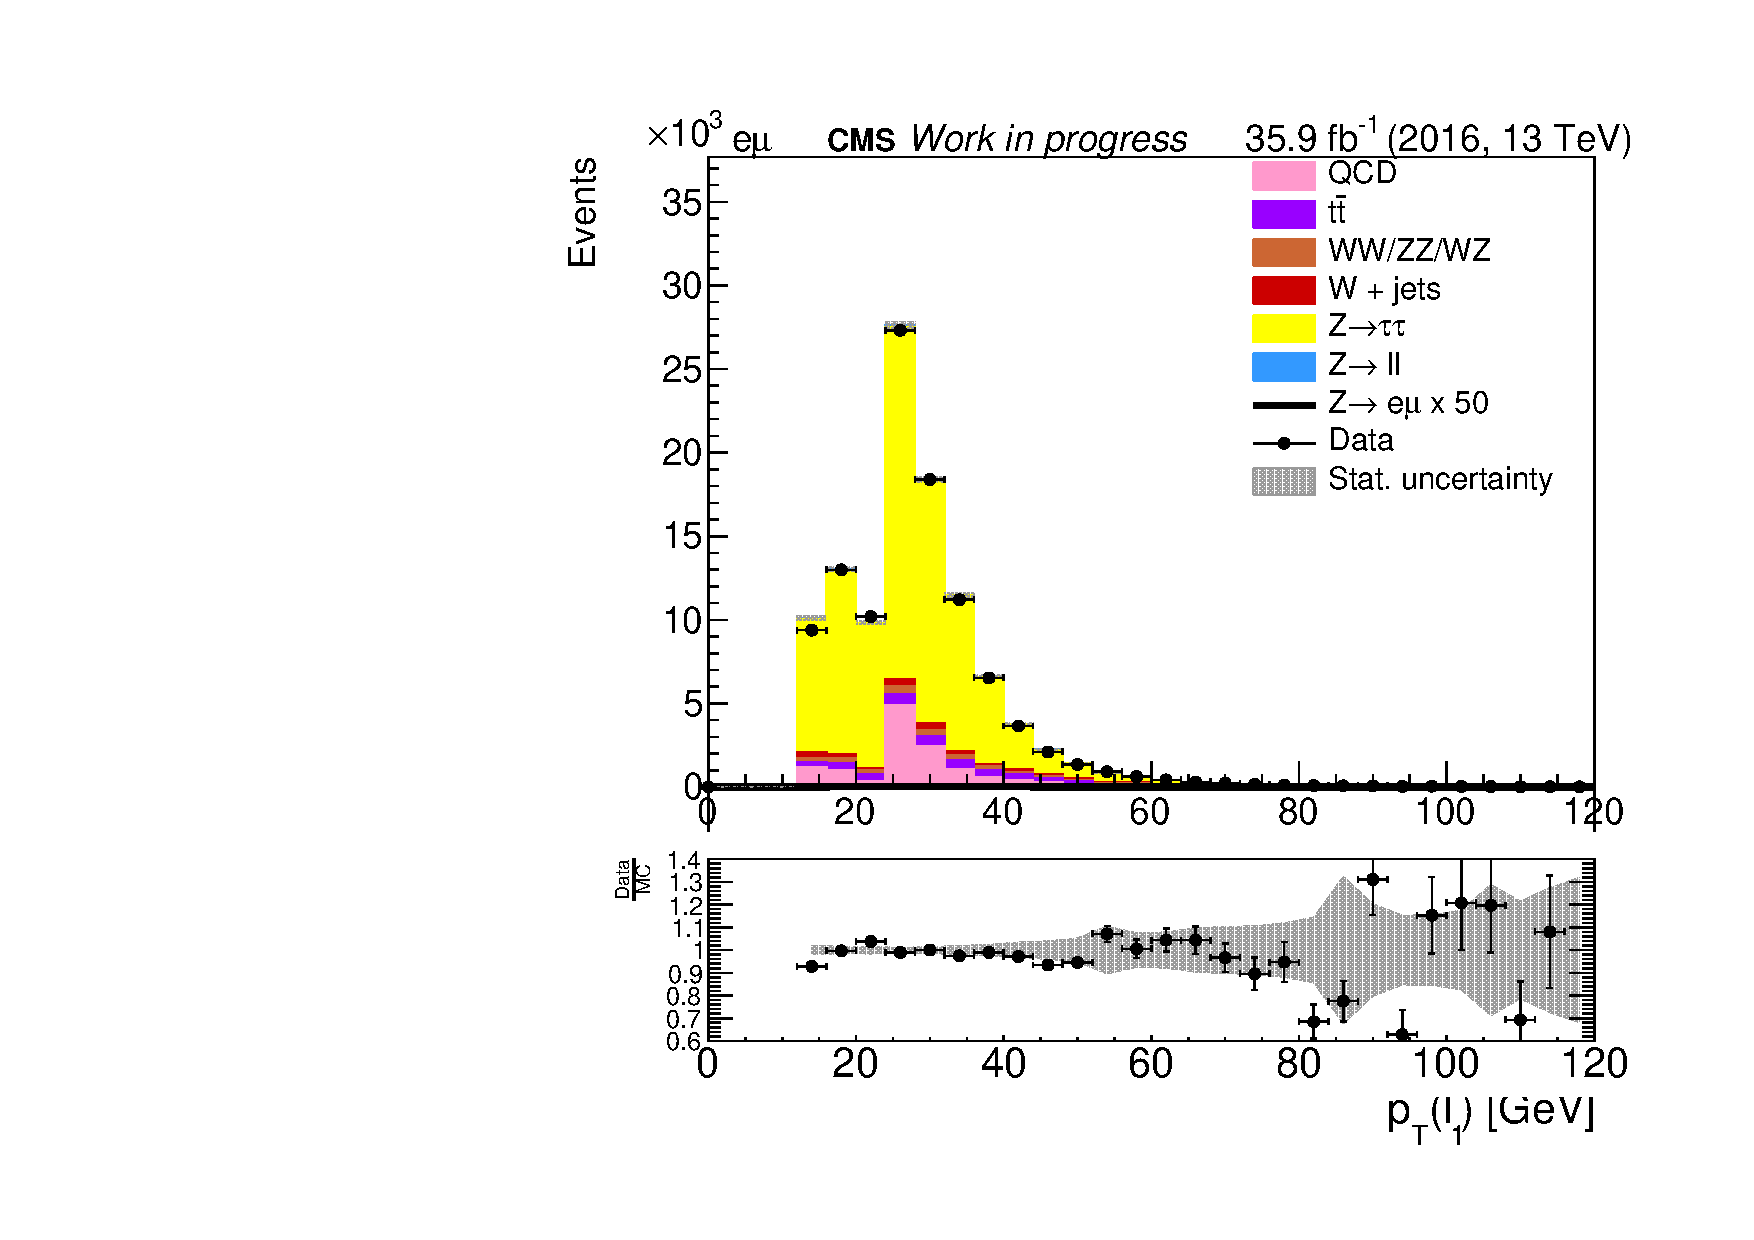
\includegraphics[width=0.4\textwidth]{plots/em/TransverseMomentum1_ZTTCR.pdf}
	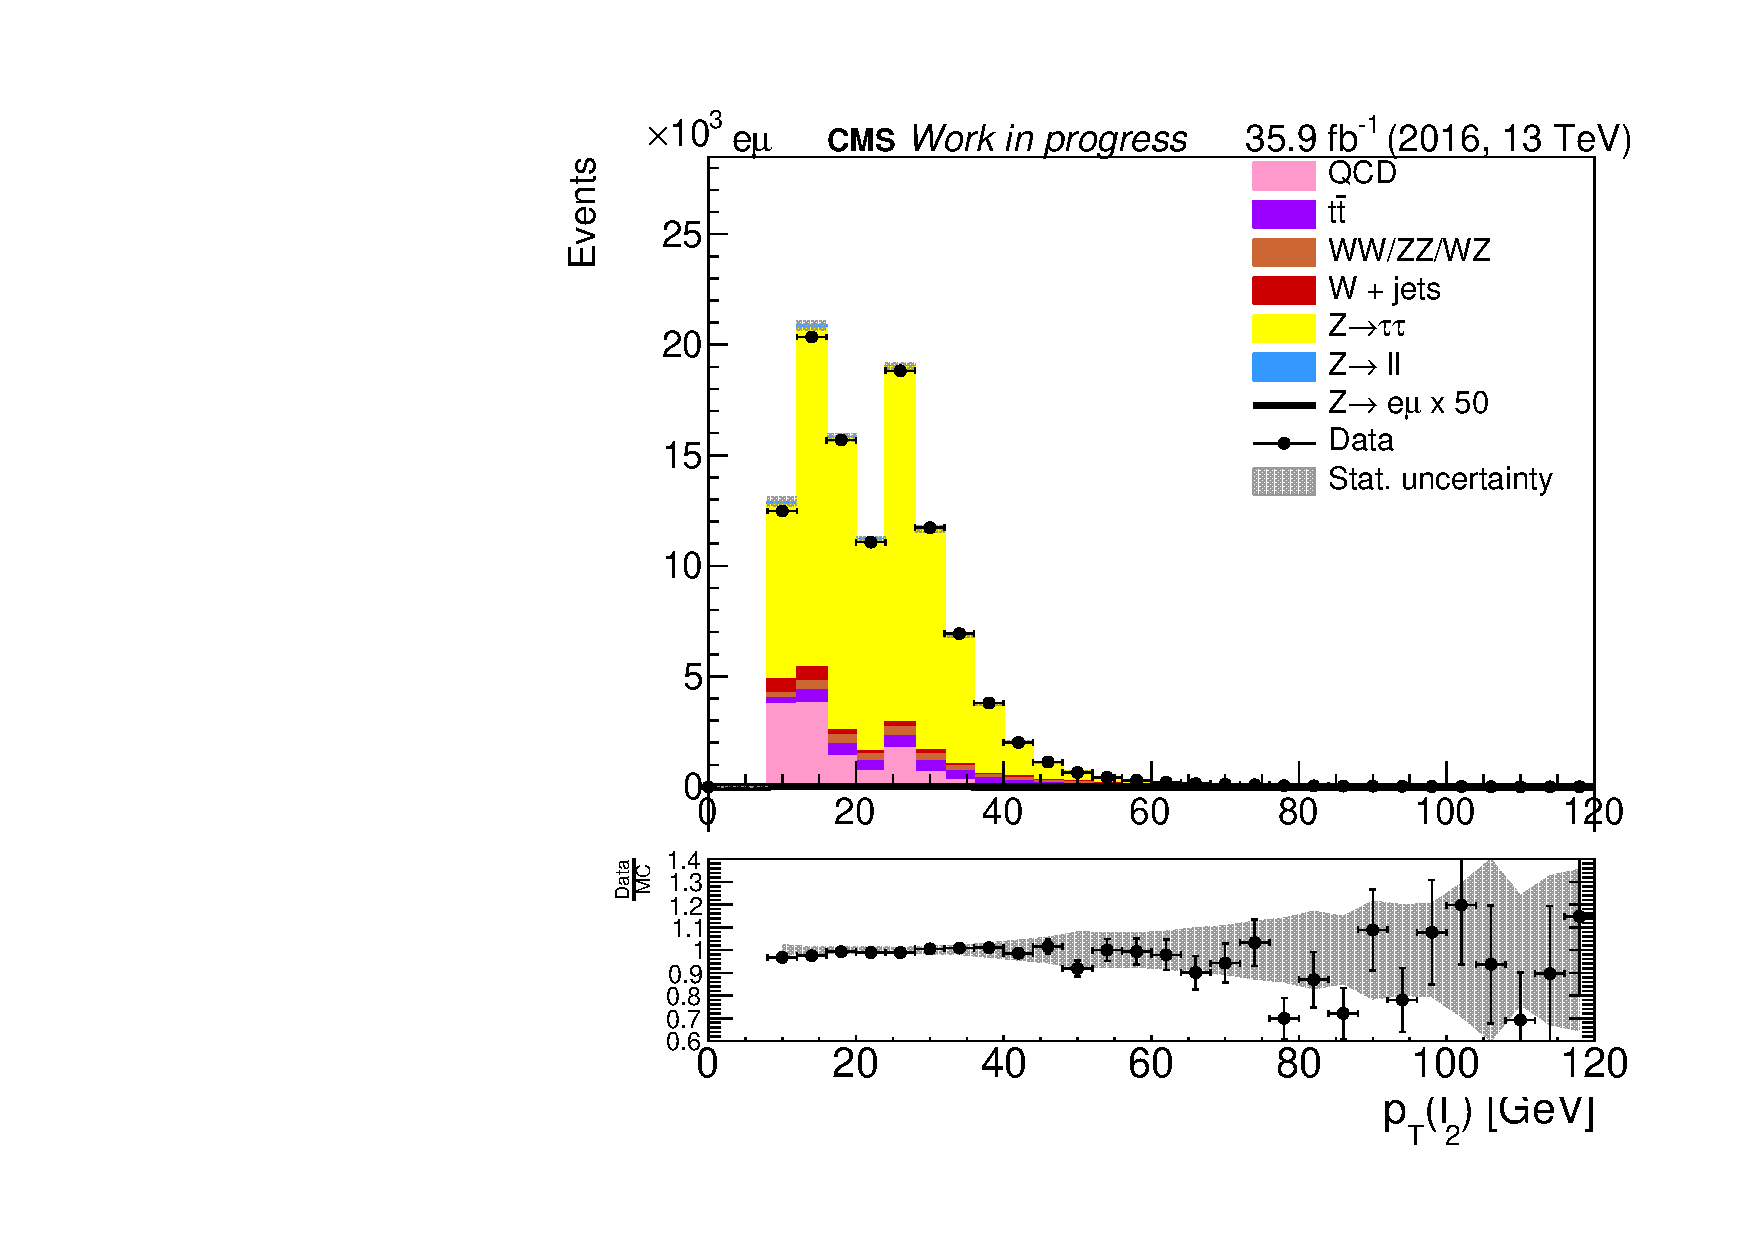
\includegraphics[width=0.4\textwidth]{plots/em/TransverseMomentum2_ZTTCR.pdf}
	
	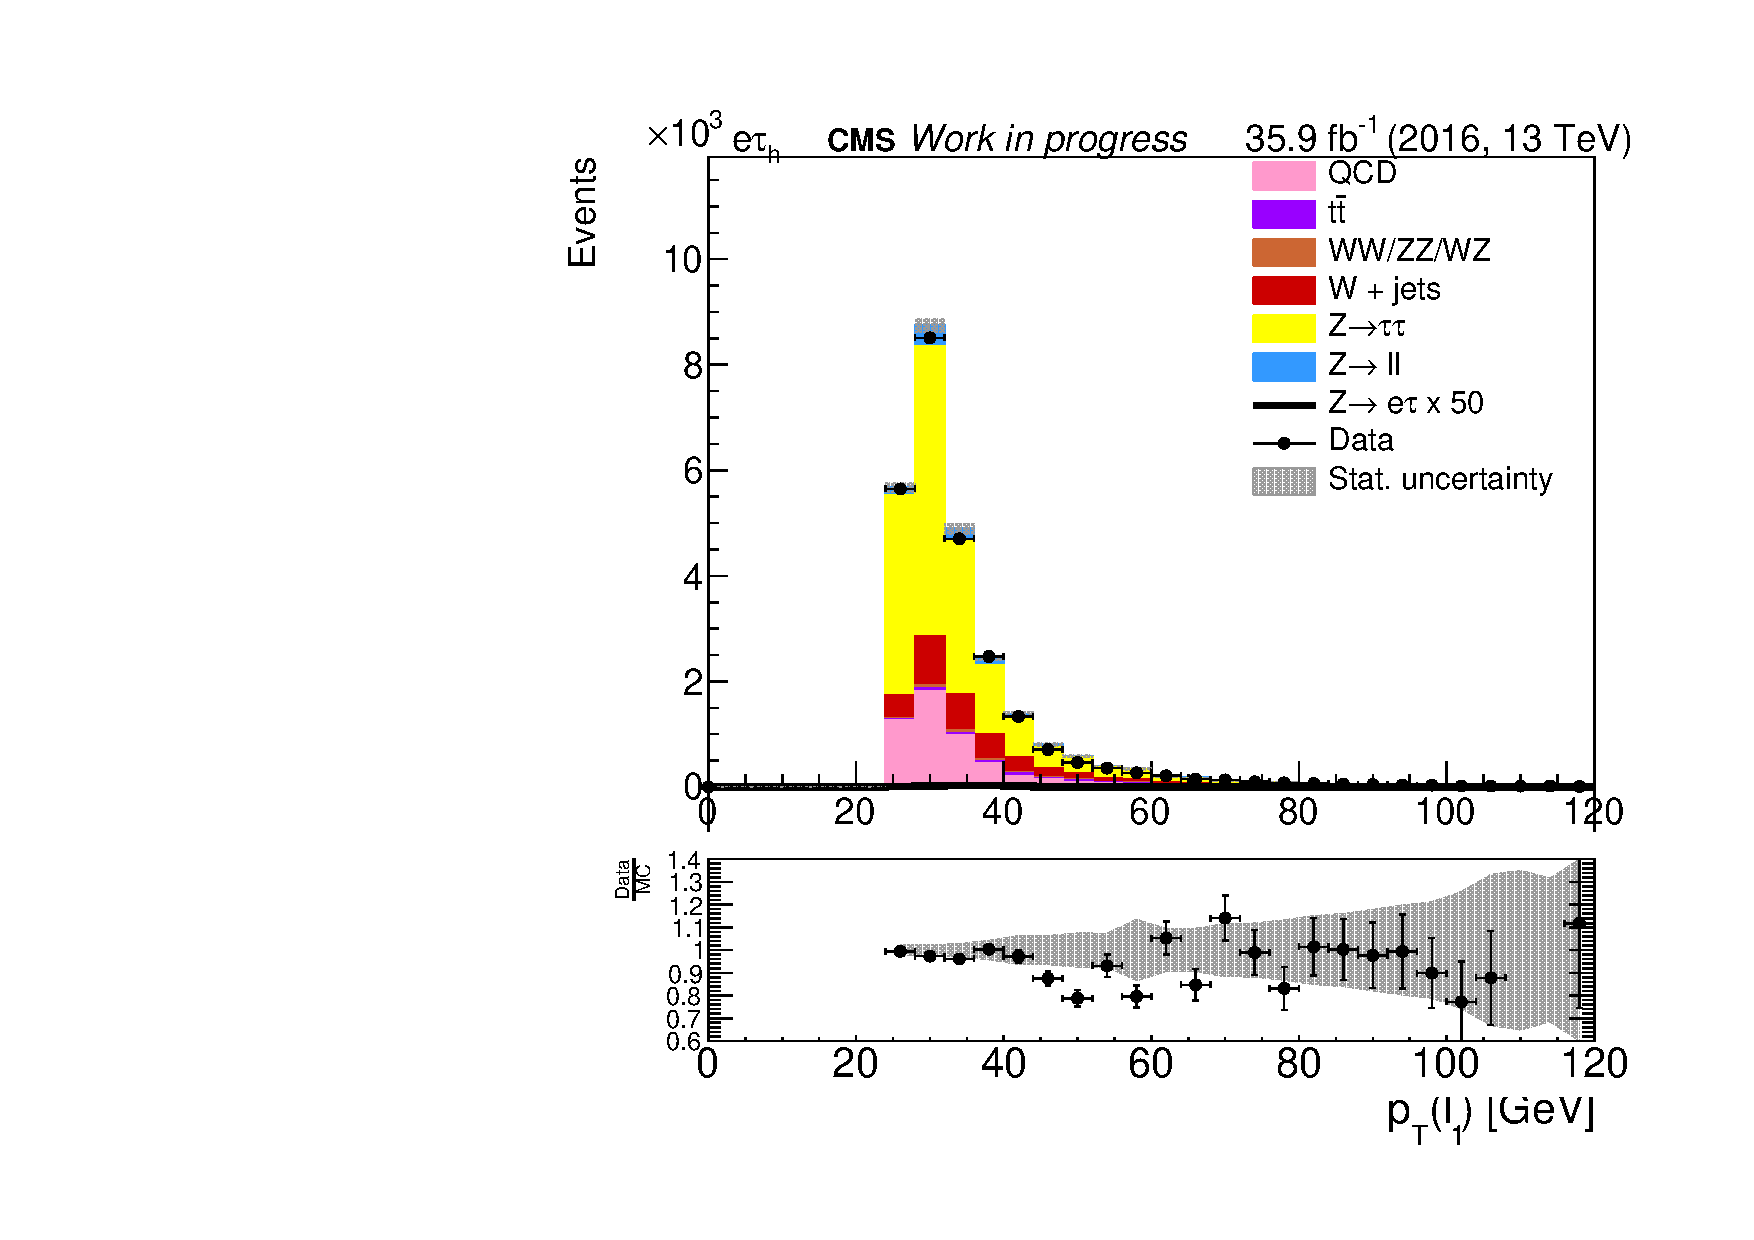
\includegraphics[width=0.4\textwidth]{plots/et/TransverseMomentum1_ZTTCR.pdf}
	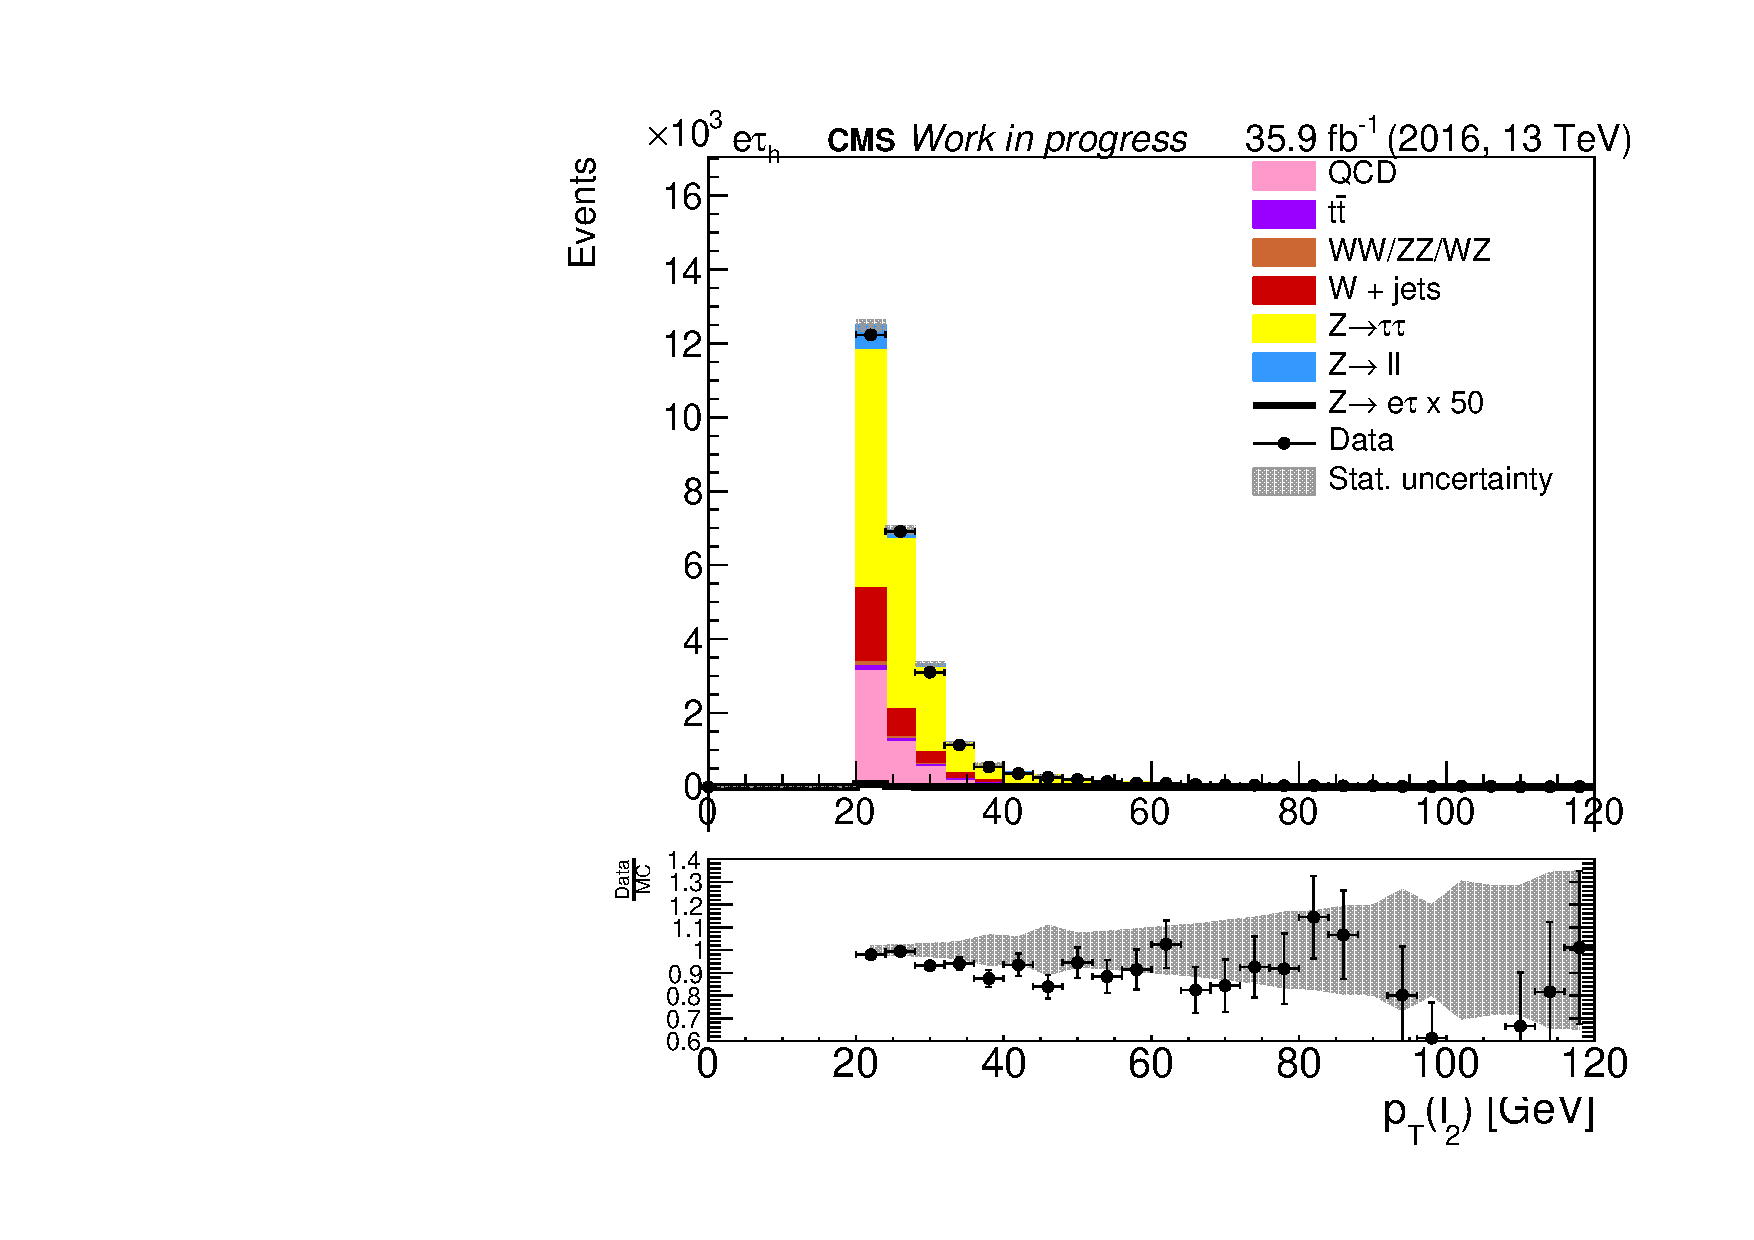
\includegraphics[width=0.4\textwidth]{plots/et/TransverseMomentum2_ZTTCR.pdf}

	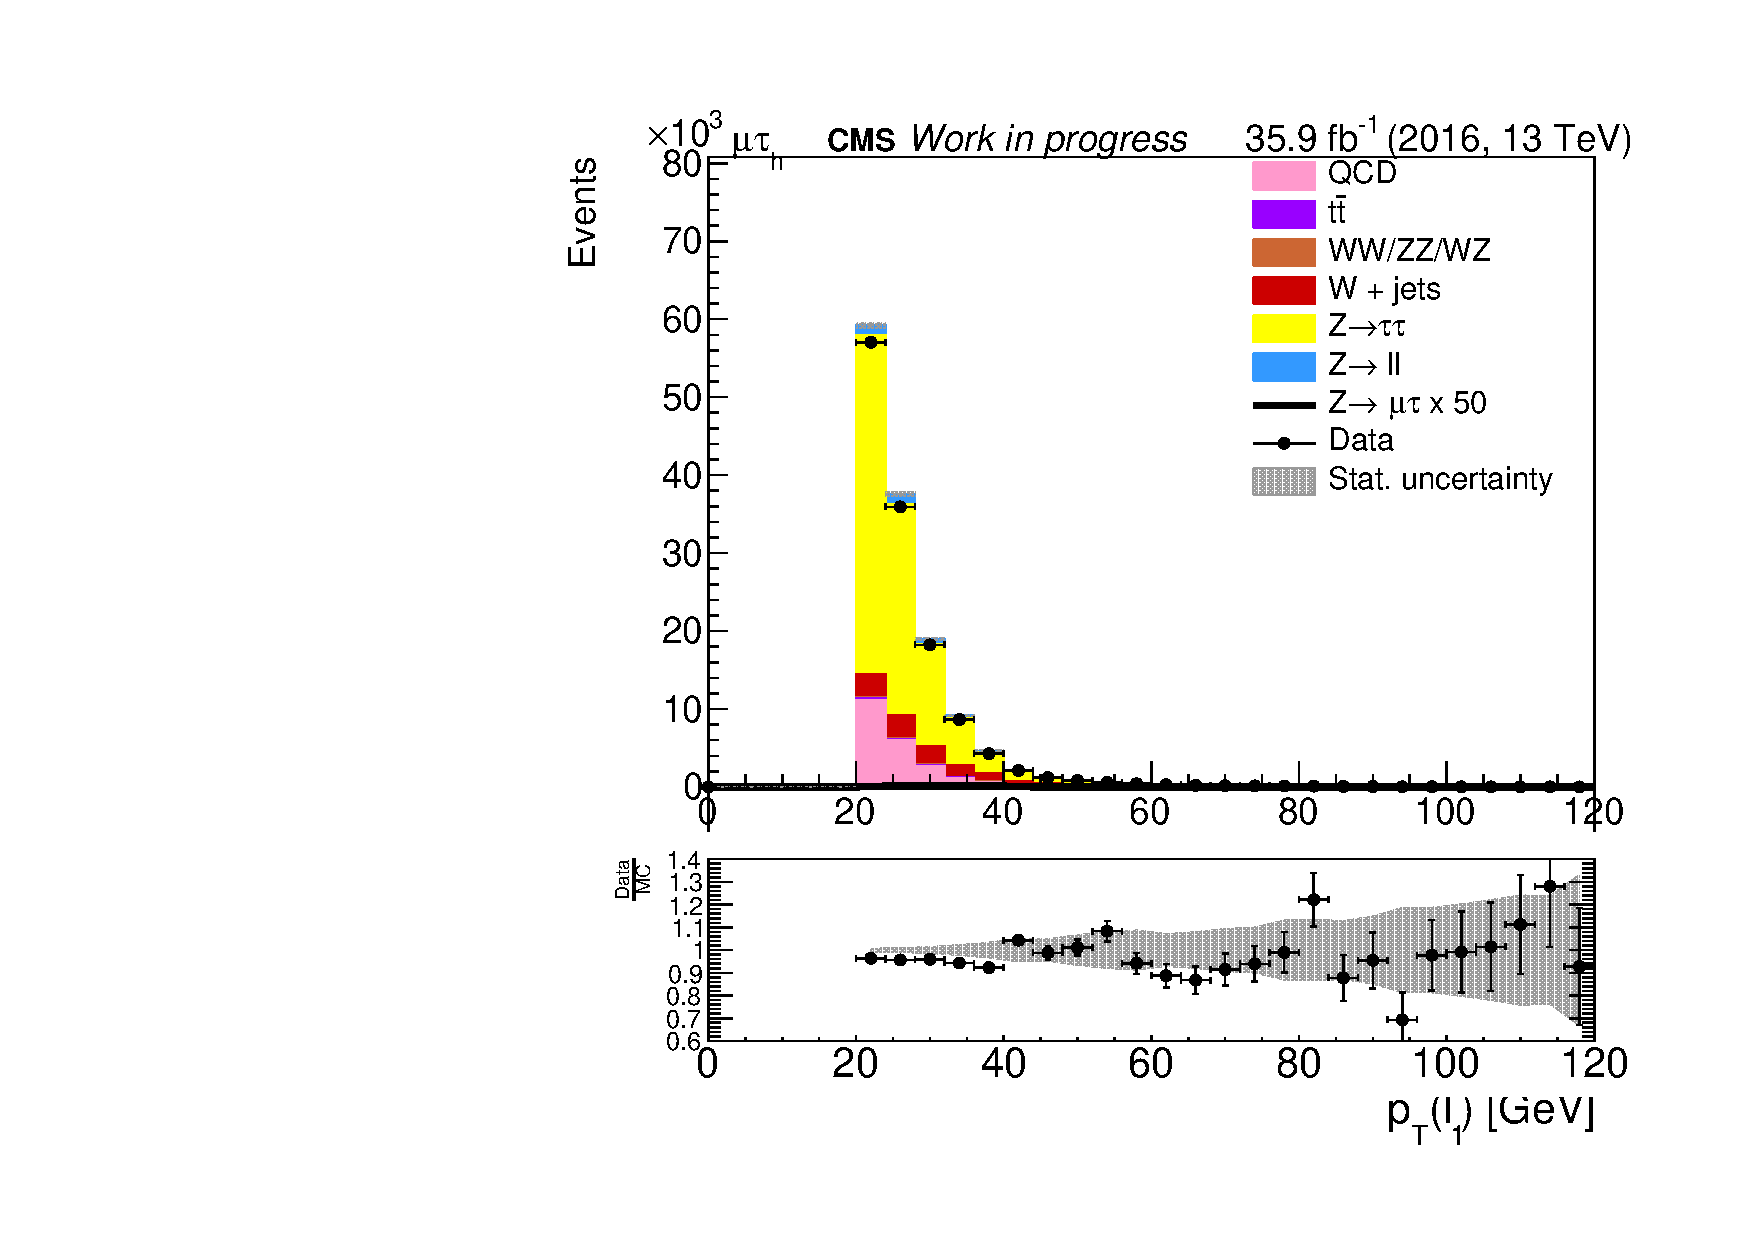
\includegraphics[width=0.4\textwidth]{plots/mt/TransverseMomentum1_ZTTCR.pdf}
	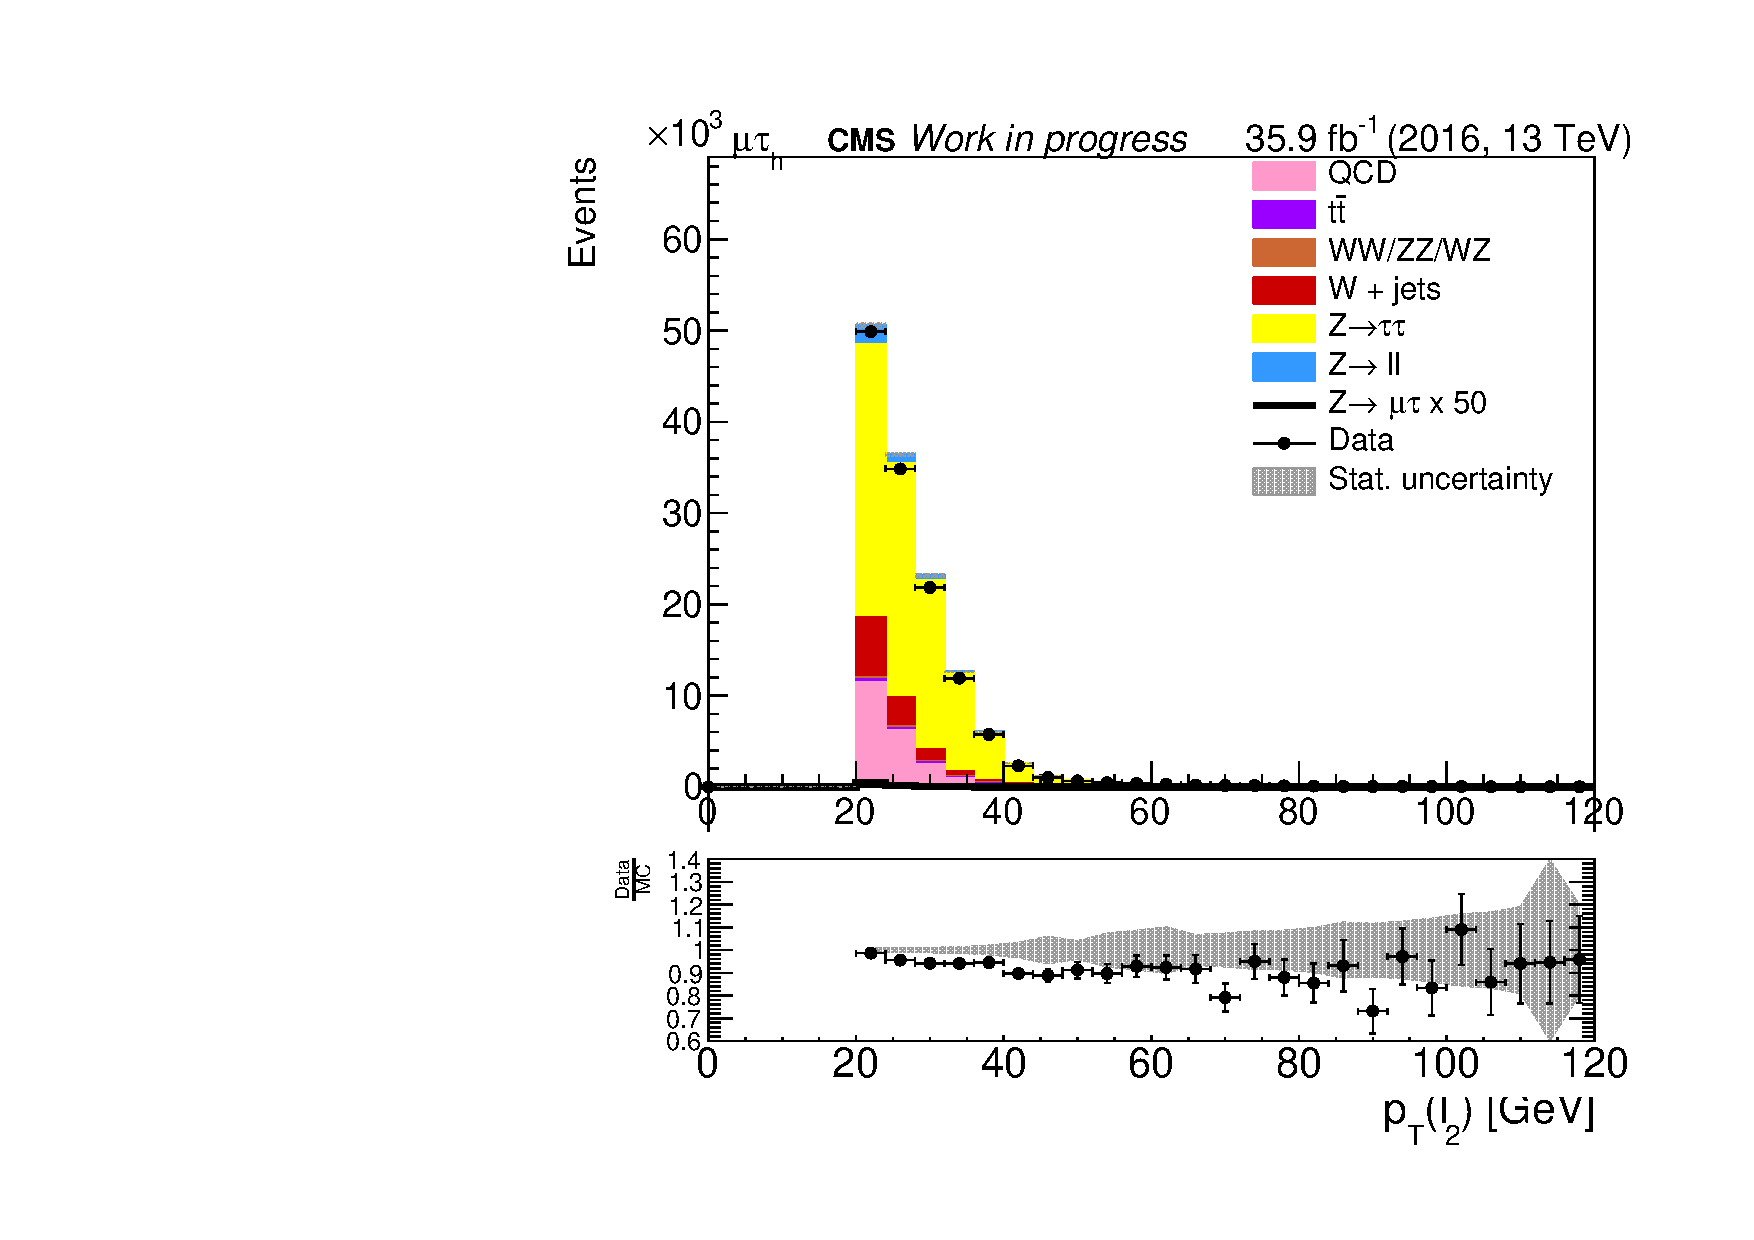
\includegraphics[width=0.4\textwidth]{plots/mt/TransverseMomentum2_ZTTCR.pdf}

	\caption[\gls{pT} distribution for $Z\to\tau\tau$ control region]{\gls{pT} distribution of both lepton for the final state $e\mu$, $e\tau$ and $\mu\tau$, where only events around the visible mass peak of $Z\to\tau\tau$ are take: 20 GeV $<$ \gls{m_vis} $<$ 60 GeV}
	\label{fig:fig_3_8}
\end{figure}

The $t\bar{t}$ and the di-boson background, including all productions modes of two vector bosons, top quark in association with a W boson and single top production, is simulated with MC and normalized to its cross section and the integrated luminosity. Figure \ref{fig:fig_3_9} shows the \gls{pT} distribution of event with two b-tagged jets, which is \gls{TTBAR} dominated.
\begin{figure}[htp]
	\centering
	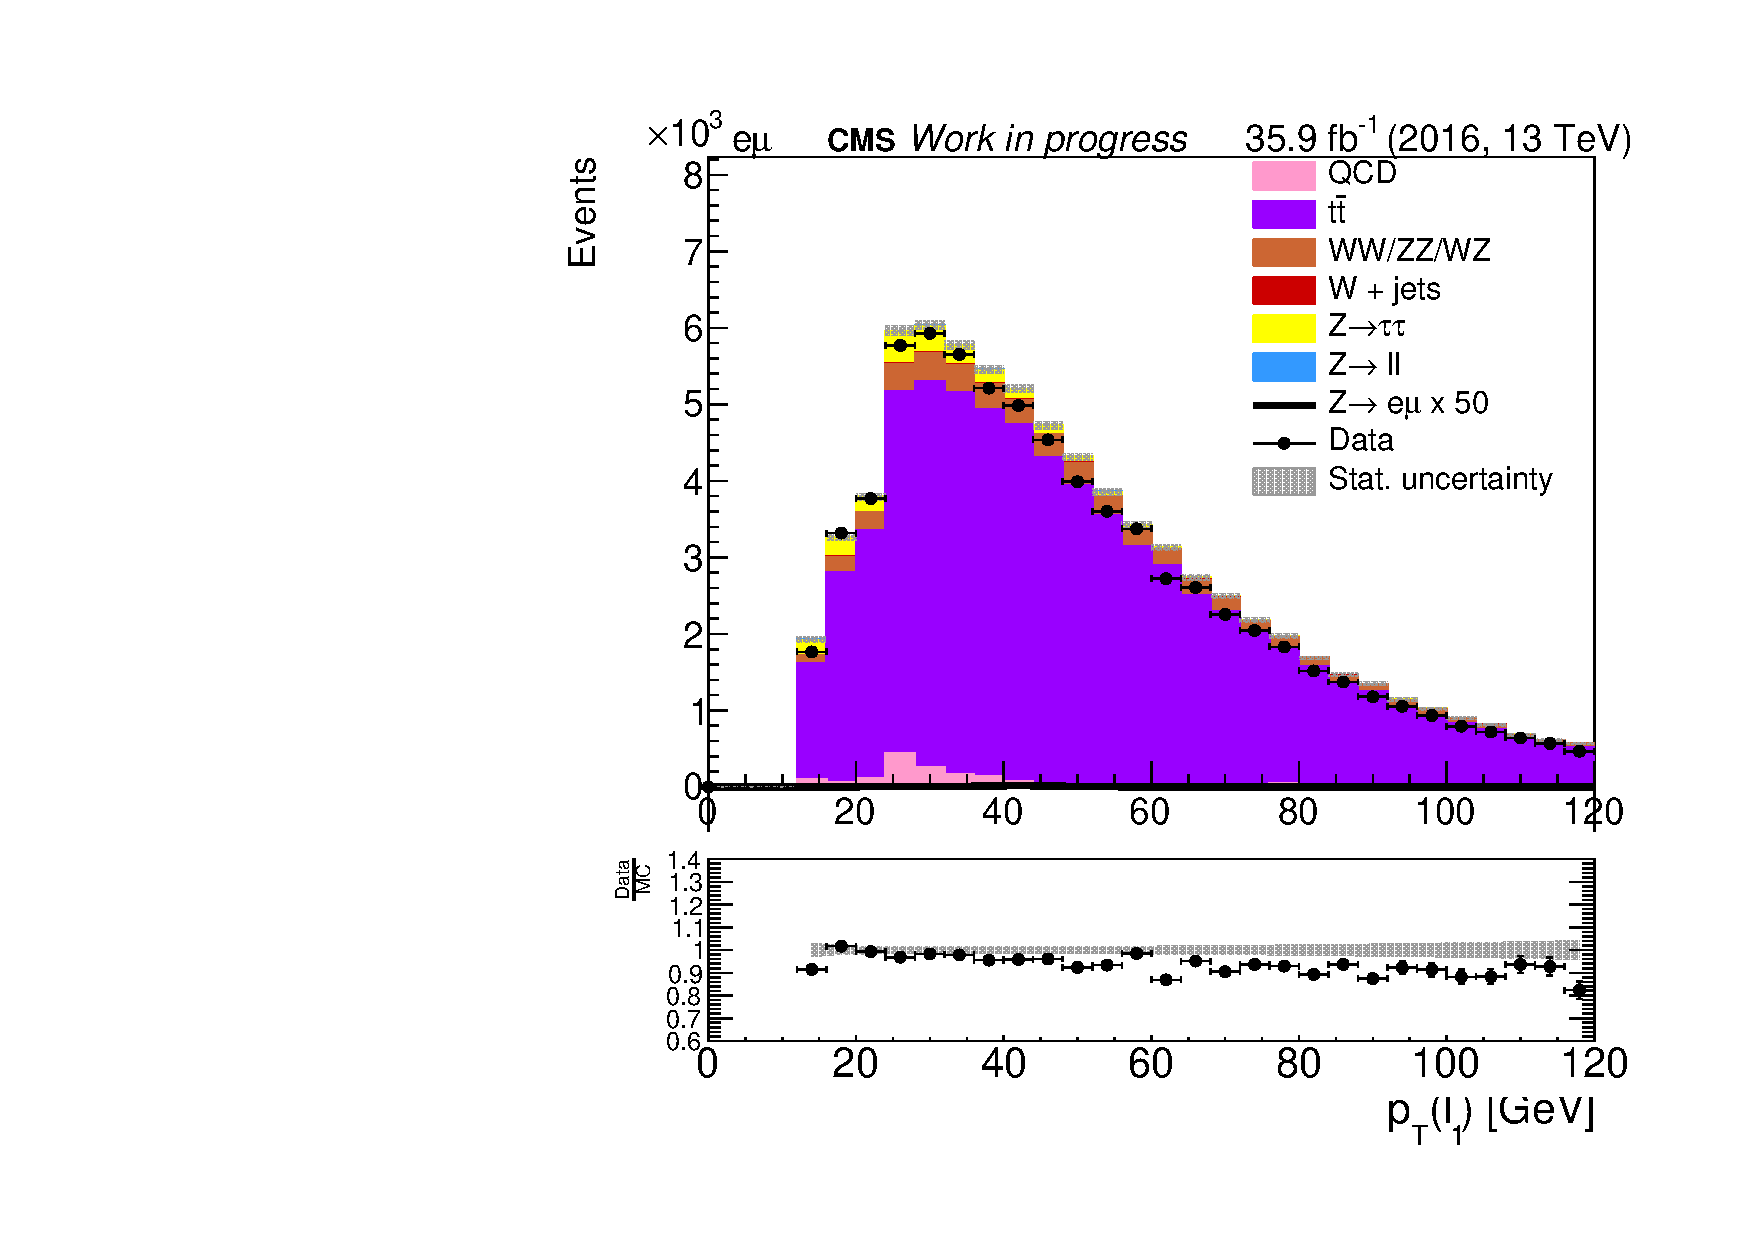
\includegraphics[width=0.4\textwidth]{plots/em/TransverseMomentum1_TTBARCR.pdf}
	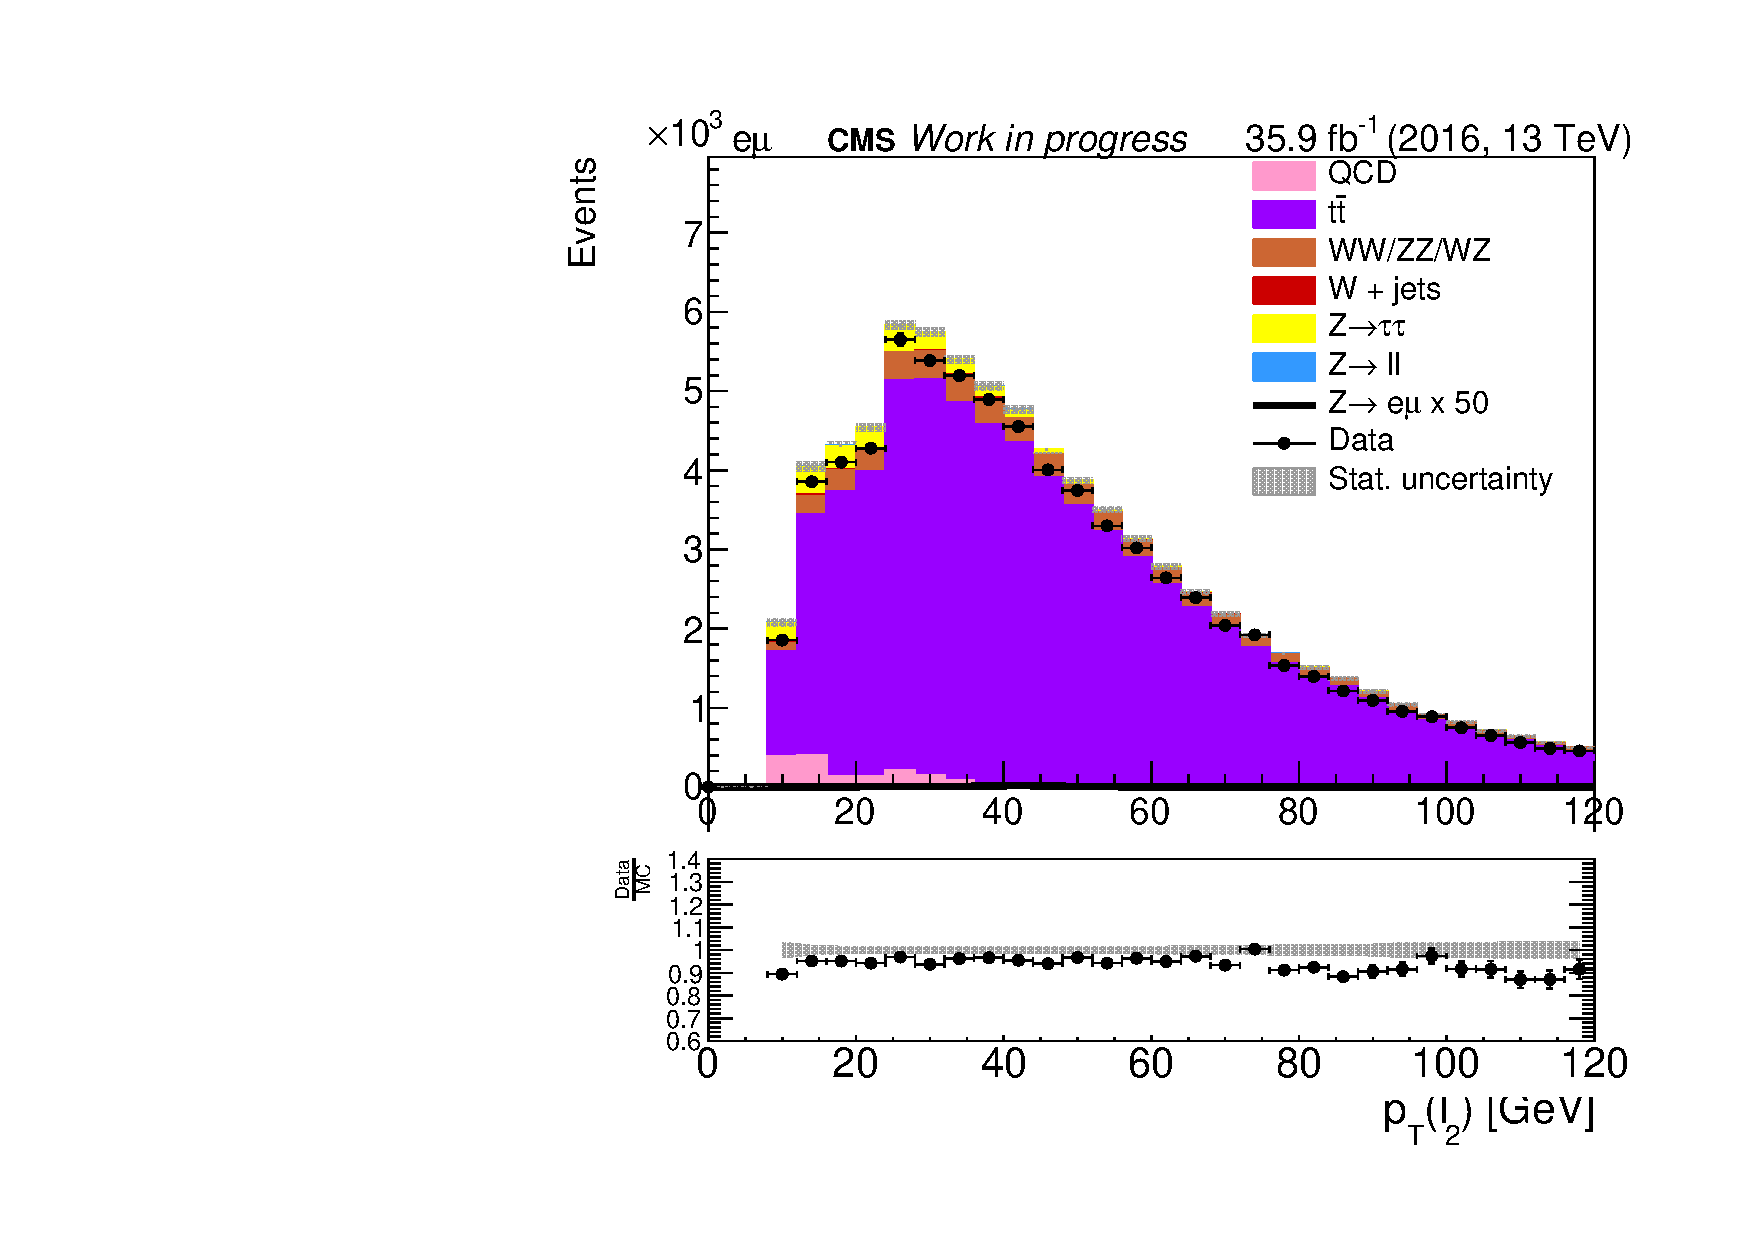
\includegraphics[width=0.4\textwidth]{plots/em/TransverseMomentum2_TTBARCR.pdf}
	
	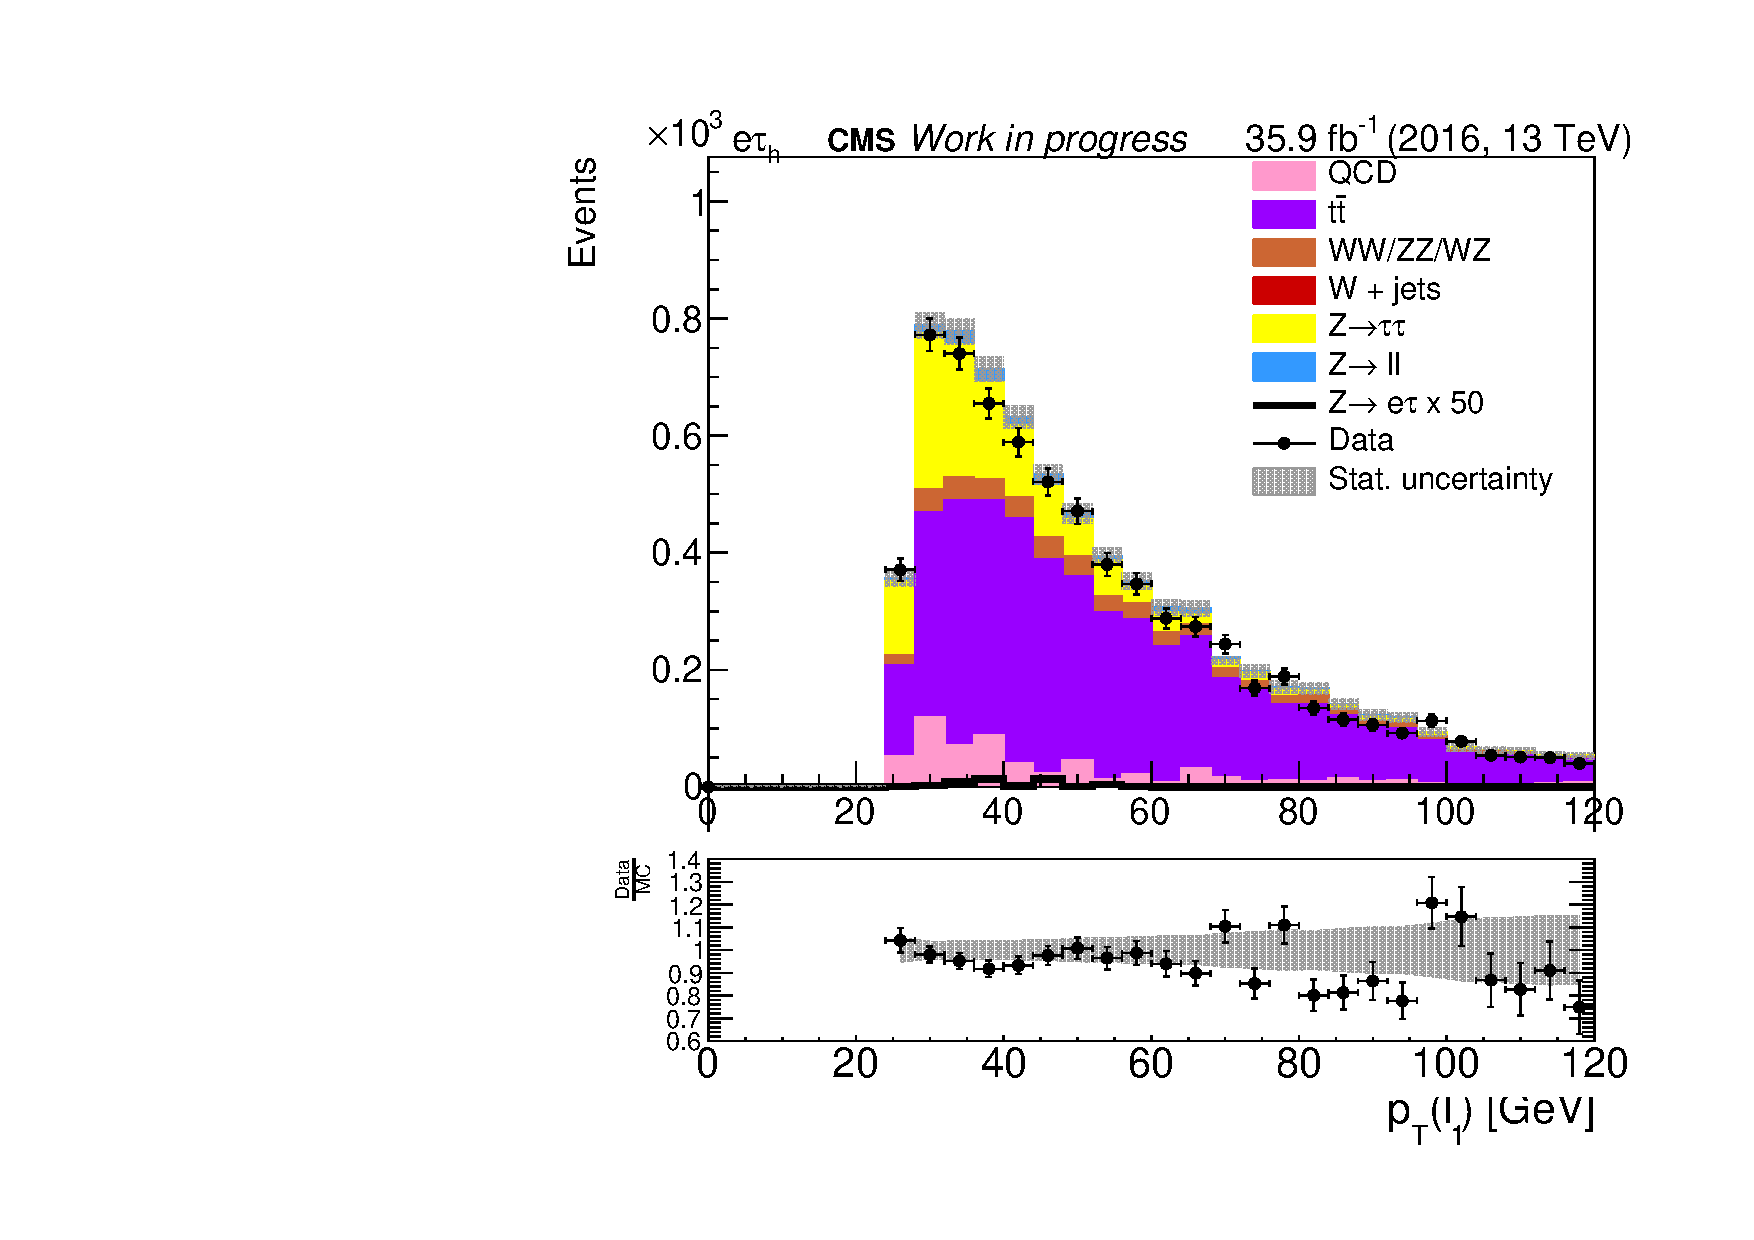
\includegraphics[width=0.4\textwidth]{plots/et/TransverseMomentum1_TTBARCR.pdf}
	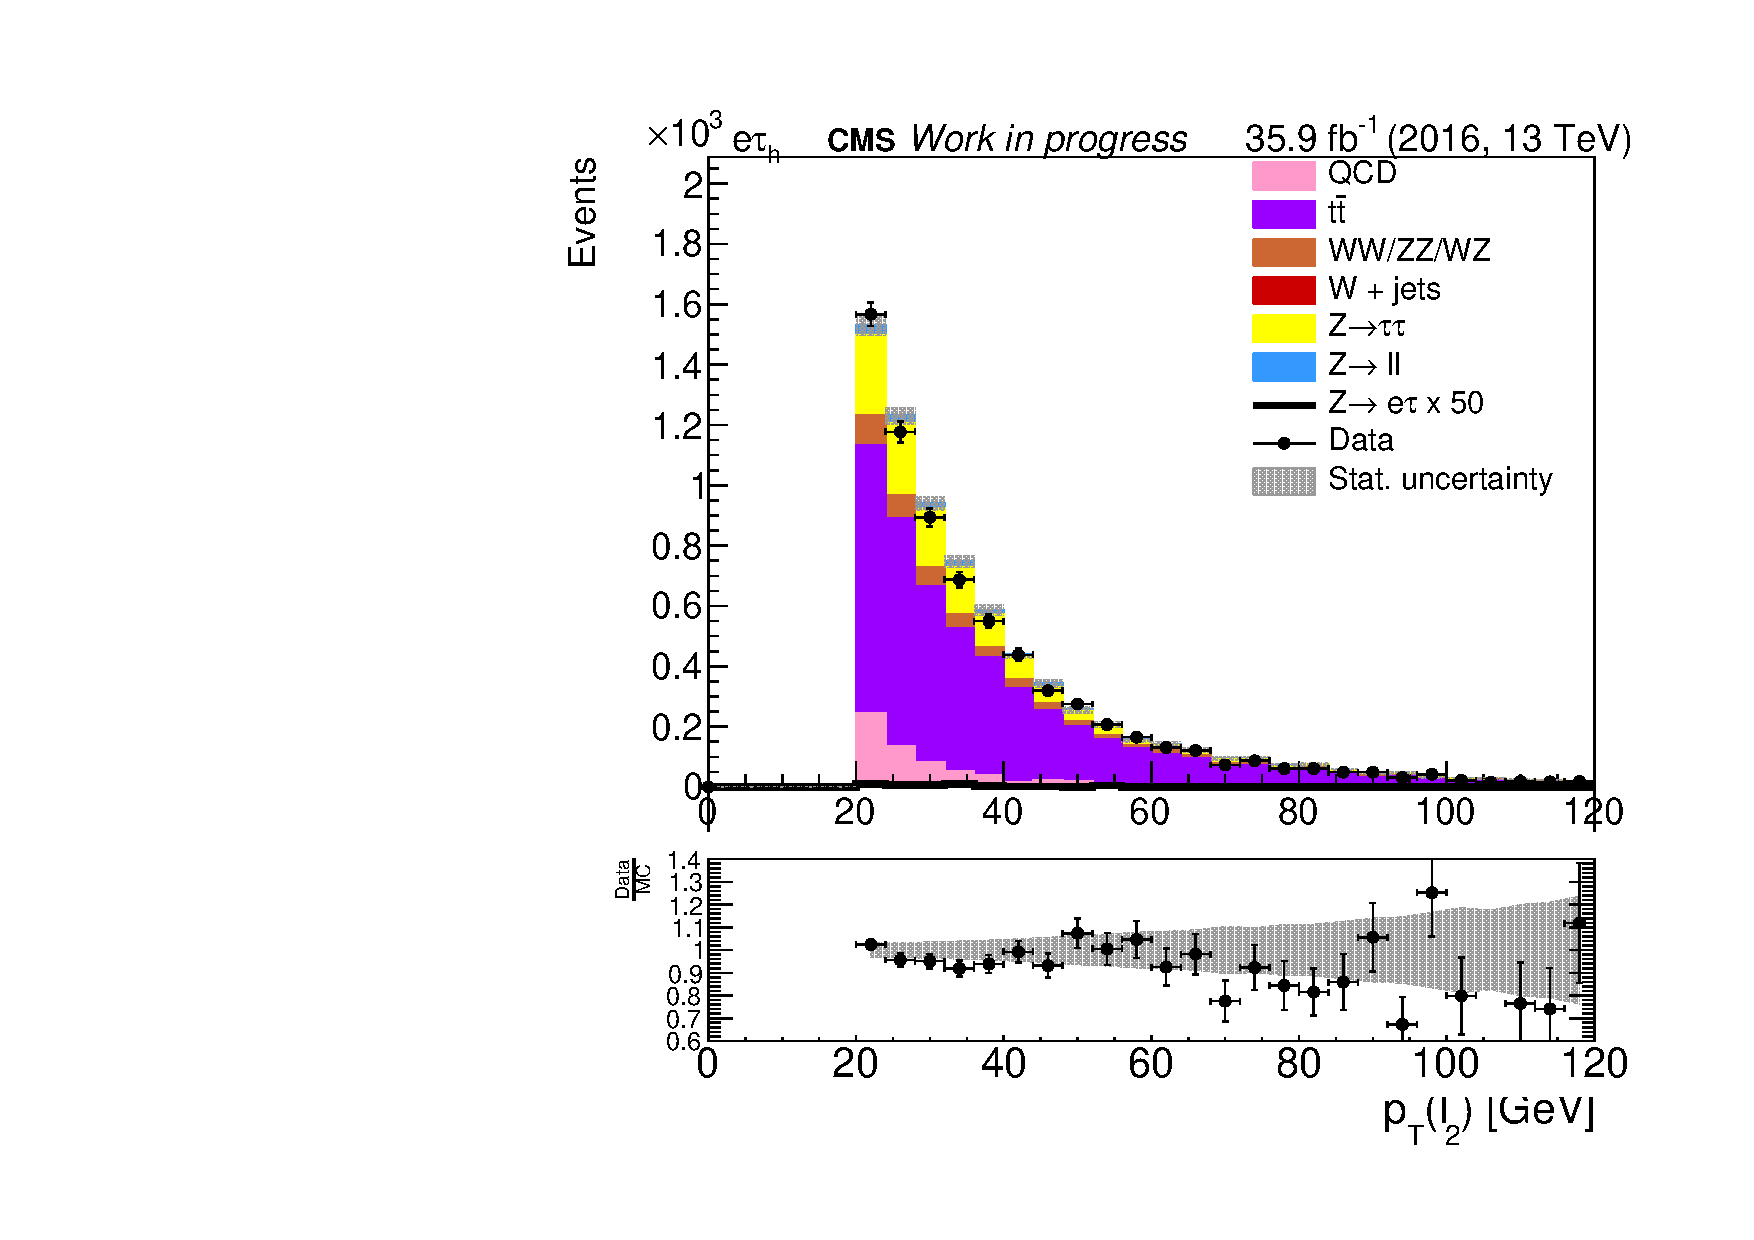
\includegraphics[width=0.4\textwidth]{plots/et/TransverseMomentum2_TTBARCR.pdf}

	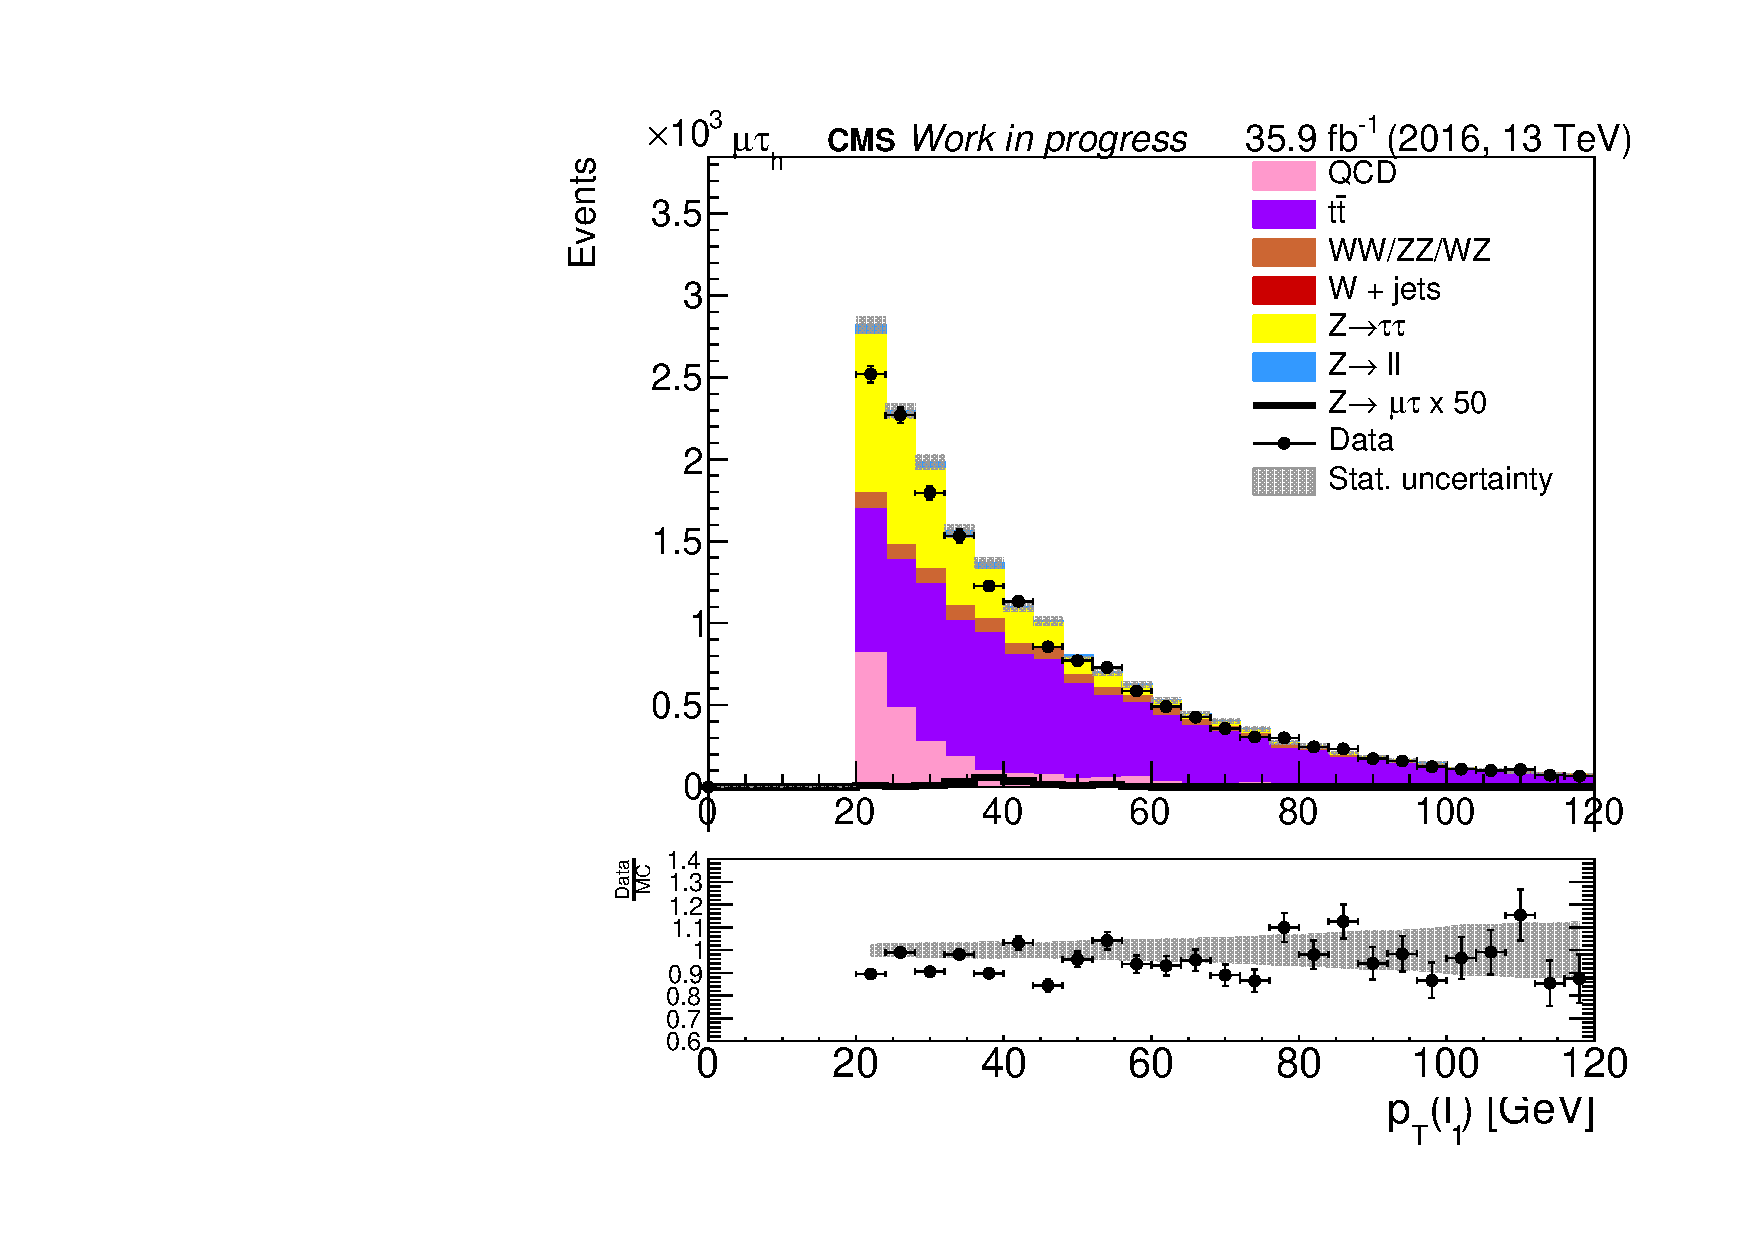
\includegraphics[width=0.4\textwidth]{plots/mt/TransverseMomentum1_TTBARCR.pdf}
	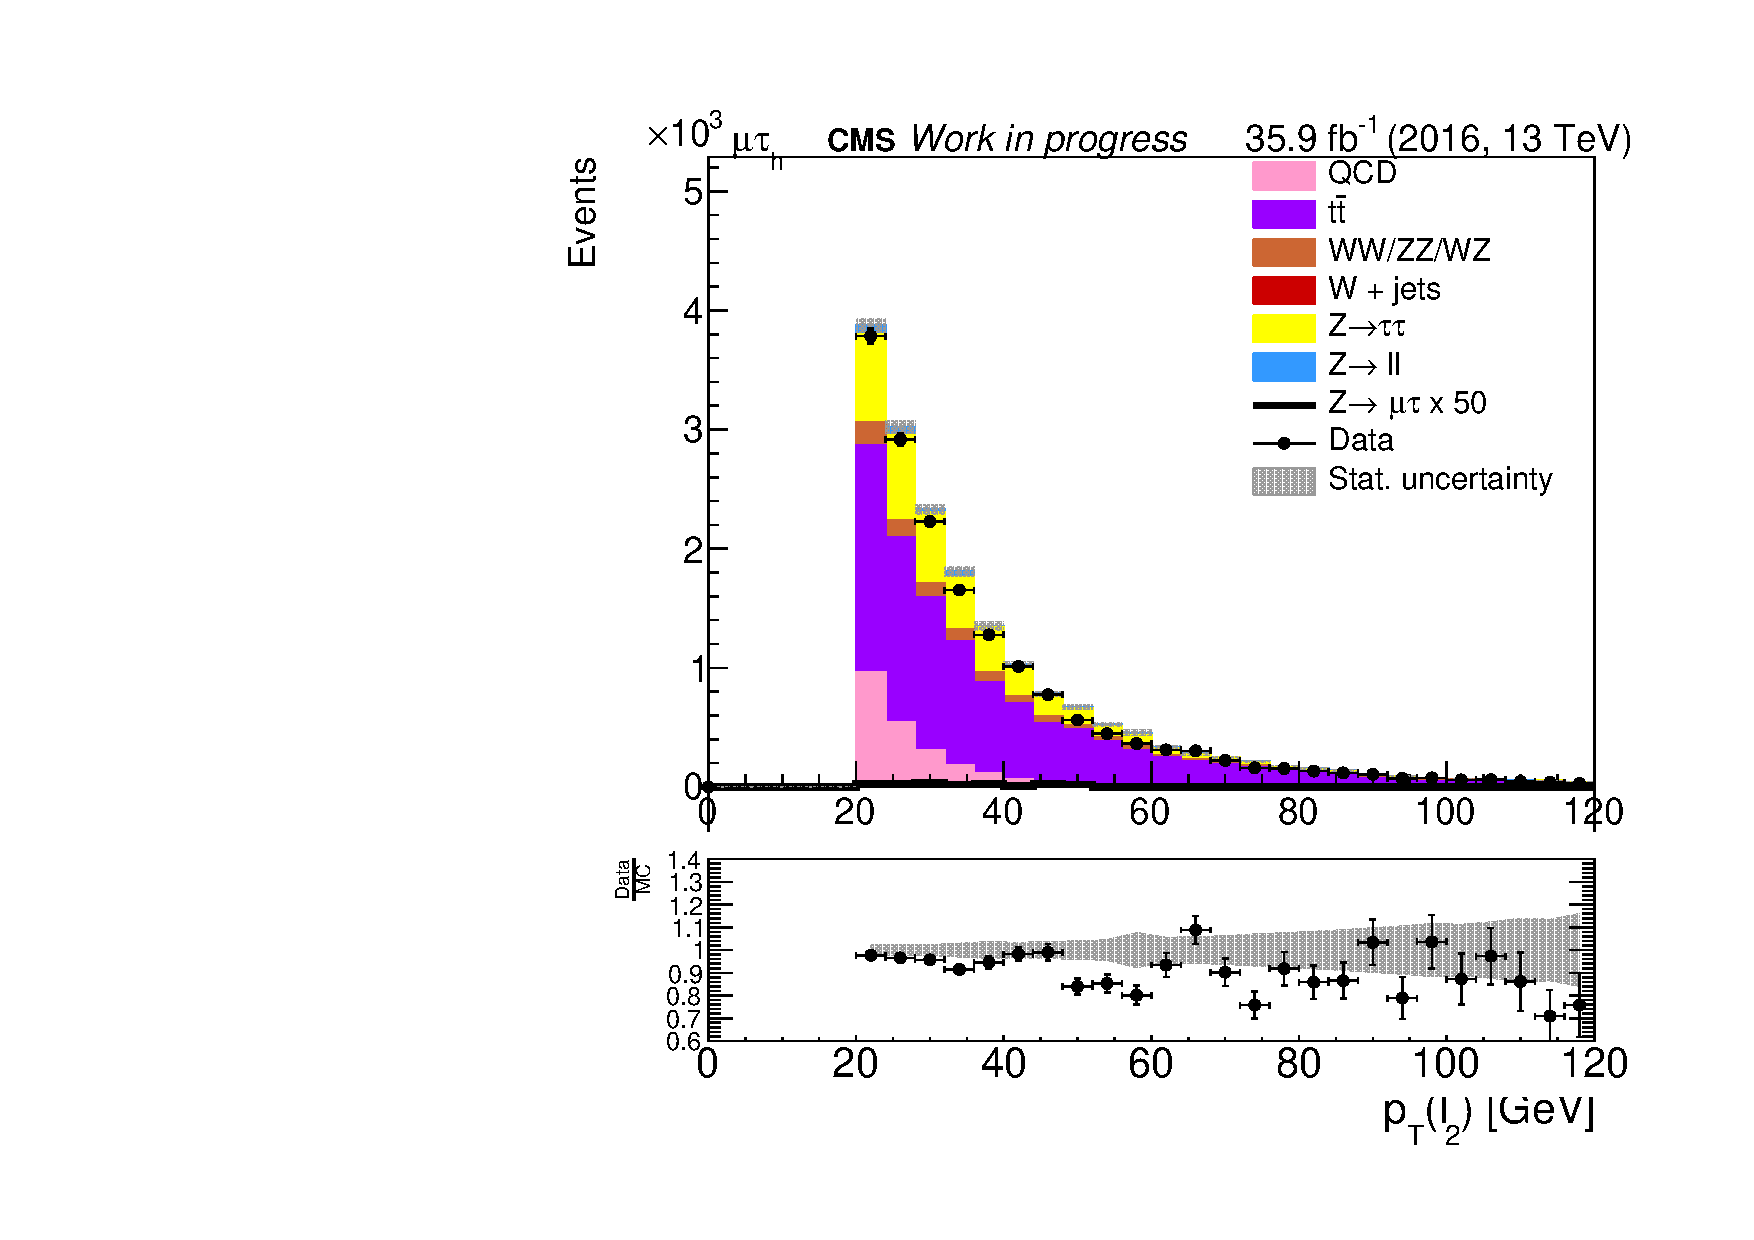
\includegraphics[width=0.4\textwidth]{plots/mt/TransverseMomentum2_TTBARCR.pdf}

	\caption[\gls{pT} distribution for \gls{TTBAR} control region]{\gls{pT} distribution of both lepton for the final state $e\mu$, $e\tau$ and $\mu\tau$, where only events with two b-tagged jets are considered}
	\label{fig:fig_3_9}
\end{figure}

\subsection{Background estimated using data driven methods}

For the $e\mu$ final state, the $W + \text{jet}$ is a minor background due to the small probability for a jet to be misidentified as an isolated lepton. Because of this reason, in this final state the estimation is done with MC simulation and normalized with cross section and integrated luminosity. The QCD shape is taken from a same-sign (SS) region, where both leptons pass relaxed isolation criterias. The normalization is extrapolated from comparing SS and opposite-sign (OS) regions, where one of the two leptons fullfill $0.3 < I^{\ell} < 0.5$. 

In the case of the $e\tau$ / $\mu\tau$ final state, $W + \text{jets}$ normalization and QCD is simultaneously estimated with a data driven method. A schematic overview of the regions used for the estimation are shown in Figure \ref{fig:mt}. The number of events in the oppositite-sign (OS) signal region (SR), which events fullfill $M_T < 50$ GeV (low $M_T$), is calculated with 

\begin{equation}
	W^{\text{low } M_T}_{OS} = (\frac{W^{\text{low } M_T}_{\text{sim. relaxed OS}}}{W^{\text{high } M_T}_{\text{sim. relaxed OS}}}) \cdot W^{\text{high } M_T}_{OS}
\end{equation}

with $W^{\text{low } M_T}_{\text{sim. relaxed OS}}$ and $W^{\text{high } M_T}_{\text{sim. relaxed OS}}$ as number of events taken from simulation, where relaxed isolation criteria is applied. For the number of events in the OS region in the control region (CR), where events fullfill $M_T > 50$GeV (high $M_T$), is extracted from data using 

\begin{equation}
	W^{\text{high } M_T}_{OS} = \text{data}^{\text{high } M_T}_{OS} - Z^{\text{high } M_T}_{OS} - t\bar{t}^{\text{high } M_T}_{OS} - \text{diboson}^{\text{high } M_T}_{OS} - \text{QCD}^{\text{high } M_T}_{OS}
\end{equation}

with data and all other backgrounds explained in the previous section. The number of events for QCD in the high $M_T$ region with OS events are estimated using

\begin{equation}
\text{QCD}^{\text{high } M_T}_{OS} = \epsilon^{QCD}_{OS/SS} \cdot (\text{data}^{\text{high } M_T}_{SS} - Z^{\text{high } M_T}_{SS} - t\bar{t}^{\text{high } M_T}_{SS} - \text{diboson}^{\text{high } M_T}_{SS} - W^{\text{high } M_T}_{\text{sim. SS}})
\end{equation}

with data and all other backgrounds explained in the sections before, including simulated $W + \text{jets}$ events, in the SS high $M_T$ CR region. The factor $\epsilon^{QCD}_{OS/SS}$ is an extrapolation from SS to OS region, which is calculated using samples with inverted isolation criteria of the leptons. Using the same extrapolation factor, the distrubtion of QCD in the low $M_T$ signal region is calculated using 

\begin{equation}
	\text{QCD}^{\text{low } M_T}_{OS} = \epsilon^{QCD}_{OS/SS} \cdot (\text{data}^{\text{low } M_T}_{SS} - Z^{\text{low } M_T}_{SS} - t\bar{t}^{\text{low } M_T}_{SS} - \text{diboson}^{\text{low } M_T}_{SS} -  (\frac{W^{\text{low } M_T}_{\text{OS}}}{W^{\text{high } M_T}_{\text{sim. OS}}}) \cdot W^{\text{low } M_T}_{\text{SS}})
\end{equation}


\subsection{Correction of simulated events}

Limited power of modelling the pp-interactions, pile up and the detector response leads to discrepancies in the \gls{MC} simulation and real data. To correct such discrepancies, scale factors and kinematic corrections are applied. In general the factors for the corrections are provided by the \gls{CMS} collaboration. \\

Trigger/and idenfitcation of particles shows different efficencies in data and \gls{MC}. With scale factors of binned in \gls{pT} and \gls{eta} this efficiences of \gls{MC} are matched to data. For the idenfication the scales factors depens on the working point of the idenfitcation selection. For the case of the \gls{TAUH}, where extra \gls{MVA} idenfications to discriminate electrons and muons are used, scale factors in bins of \gls{eta} are applied. \\

Beside selection efficiences, also correction of the measured energy/momentum has to be applied. In the case of the \gls{TAUH}, the four momenta of the is corrected by -1.8\% in the 1-prong decay mode, by +1.0\% in the 1-prong + $\pi^{0}$ decay mode and by 0.4\% in the 3-prong decay mode. To correct the energy scales of electrons/muons faking a \gls{TAUH} the four momenta of \gls{TAUH}, which are gen matched to an electron or muon, are corrected. For a gen matching to a muons a correction of -0.2\% for the 1-prong decay mode and of +1.5\% for the 1-prong + $\pi^{0}$ decay mode is applied. For a gen matching to an electron a correction of 9.5\% in the 1-prong + $\pi^{0}$ decay mode is applied. \\

For the jet energy scale by a factorized approach, where scale factors on the jet four momenta are applied. The \gls{MET} is corrected by a Type-I correction, which propagates the jet energy corrections through the calculation of the MET. For the Z boson and top quark, \gls{pT} corrections are applied. \\

For $Z\to\tau\tau$ corrections are calculated from a $Z\to\mu\mu$ control sample, where 2D scale factors in \gls{pT} and \gls{m_vis} are calculated like in the in the SM $H\to\tau\tau$ analysis. \cite{CMS-PAS-HIG-16-043}. For the corrections of \gls{TTBAR}, scale factor depending on the generated top \gls{pT} are applied.


\section{Boosted decision trees}

	

































